\documentclass[10pt]{article}
\usepackage[margin=1in]{geometry}
 \usepackage{auto-pst-pdf}
\usepackage{graphicx}
%\usepackage{arydshln}
\usepackage{ifpdf}
\ifpdf
  \usepackage{epstopdf}
\fi
\usepackage{multirow}
\usepackage{epsfig}
\usepackage{float}
\usepackage{url}
\usepackage{color}
\usepackage{subfigure}

%\newcommand\solidrule[1][1cm]{\rule[0.5ex]{#1}{.4pt}}
%\newcommand\dashedrule{\mbox{%
%  \solidrule[2mm]\hspace{2mm}\solidrule[2mm]\hspace{2mm}\solidrule[2mm]}}
  
%\usepackage{hyperref}

\begin{document}
\title{A Comprehensive Study of Characterizing Program Execution Time}

\author{
Young-Kyoon Suh\\
%Department of Computer Science \\
%University of Arizona \\
%\small\tt yksuh@cs.arizona.edu
}
\maketitle

%\begin{abstract}
%(Tentative) Measuring execution time is a useful tool in evaluating the performance of a program. 
%But it is challenging to obtain precise, accurate program execution time due to the presence of various system daemons 
%and their unpredictable activities. Such activities significantly contribute to varying program execution time.
%It will be very useful to predict the concrete performance of a program with different input sizes in a real situation, 
%if a (probabilistic) distribution of the execution times of that program is found, considering the daemon activities.
%%However, it is not easy to find such a characterization of the execution times. 
%In this work, we discuss several interesting phenomenon observed to characterize program execution times.
%We find that such a distribution of the execution times cannot be uniquely identified, and it will 
%be more likely to be mixture of two or more models formed by different periodicity of different daemon processes. 
%Finally, we discuss some remaining issues that should be resolved to successfully 
%identify a distribution of program execution times. 
%\end{abstract}

\section{Experiment Notes}
%% done
\begin{table}[h]
\begin{center}
\begin{tabular}{|p{3cm}||p{9cm}|p{4cm}|} \hline
Task Length & Description & Time Length\\ \cline{1-3}
%\multicolumn{3}{|c|}{Regular INC experiment. Refer to Sections~\ref{sec:emp4_summary},~\ref{sec:empv4_hist}, and~\ref{sec:empv5_hist}.} \\ \hline
INC1$\sim$INC64 & Runs of 1000 samples (on {\tt sodb12}). & 2013-10-14 $\sim$ 2013-10-15\\ \hline
INC128$\sim$INC2048 & Runs of 300 samples (on {\tt sodb12}). & 2013-12-12 $\sim$ 2013-12-21\\ \hline 
INC4096 & A run of 300 samples (on {\tt sodb12}). & 2014-06-23 $\sim$ 2014-07-10 \\ \hline 
INC4096 & A run of 40 samples (on {\tt sodb12}). & 2015-05-07 $\sim$ 2015-05-09  \\ \hline 
%INC8192 & Runs of 40/260 samples (on {\tt sodb12}). & 2015-04-23 $\sim$ 2015-04-27 / 2015-10-31 $\sim$ 2015-11-24\\ \hline
INC8192 & Runs of 40 samples (on {\tt sodb12}). & 2015-04-23 $\sim$ 2015-04-27\\ \hline
%INC16384 & Runs of 40/260 samples (on {\tt sodb12}). & 2015-04-23 $\sim$ 2015-04-23 / 2015-11-25 $\sim$ 2016-01-14\\ \hline 
INC16384 & Runs of 40 samples (on {\tt sodb12}). & 2015-04-23 $\sim$ 2015-04-23 \\ \hline 
\end{tabular}
\end{center}
\vspace{-.2in}
\caption{Notes on the regular INC data used for the histograms\label{tab:exp_notes1}}
\end{table}

%\clearpage
%\newpage

\section{Measurement Quality~\label{sec:meq}}

\begin{figure}[htp!]
	\centering
	\subfigure[Standard Deviations of PT]{
		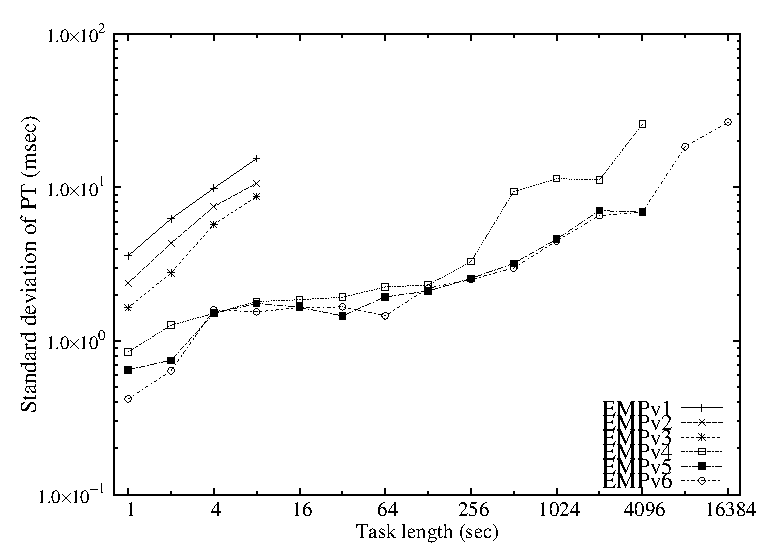
\includegraphics[scale=0.6]{overall_pt_std.eps}
        \label{fig:pt_std}
    }
    \subfigure[Relative Errors of PT]{
        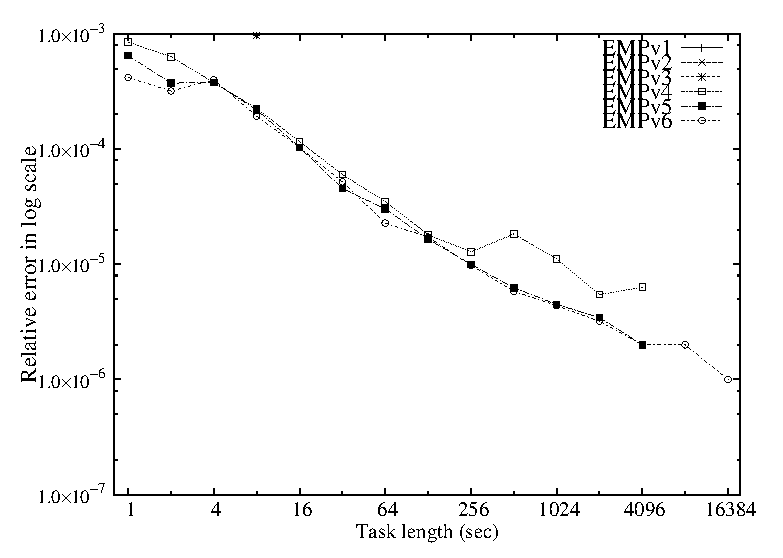
\includegraphics[scale=0.6]{overall_pt_re.eps}
        \label{fig:pt_re}
    }
    \caption{Measurement Quality Comparison among the EMP versions: updated with INC4096's another run}
    \label{fig:emp_comp}
\end{figure}

%\newpage

%\section{Summary of the EMPv4 data~\label{sec:emp4_summary}}

%\begin{table}[h]
%\centering
%{
% \begin{tabular}{|l|c|c|c|c|c|c|} \hline
%\multirow{2}{*}{}   & Num. of Samples & Minimum & Maximum & Average & Std. Dev. \\ 
%                        & & (msec)  & (msec)  & (msec)  & (msec) \\ \hline
% INC1  & 1,000 & 999.0 & 1,005.0 & 1,002.4 & 0.73\\ \hline
%
% INC2 & 1,000 & 1,996.0 & 2,007.0 & 2,004.5 & 1.38 \\\hline
%
% INC4 & 1,000 & 4,004.0 & 4,012.0 & 4,008.6 & 1.64\\\hline
%
% INC8 & 1,000 & 8,014.0 & 8,023.0 & 8,018.1 & 1.72 \\\hline 
%
% INC16 & 1,000 & 16,029.0 & 16,041.0 & 16,034.3 & 1.86 \\ \hline
%
% INC32 & 1,000 & 32,064.0 & 32,084.0 & 32,068.2 & 2.05 \\ \hline 
%
% INC64 & 1,000 & 64,129.0 & 64,145.0 & 64,135.0 & 2.27 \\ \hline 
%
% INC128 & 300 & 128,244.0 & 128,260.0 & 128,251.2 & 2.32\\ \hline
%
% INC256 & 300 & 256,494.0 & 256,523.0 & 256,502.3 & 3.29\\ \hline
%
% INC512 & 300 & 512,995.0 & 513,152.0 & 513,005.1 & 9.41\\ \hline
%
% INC1024 & 300 & 1,025,997.0 & 1,026,141.0 & 1,026,012.4 & 11.43\\ \hline
%
% INC2048 & 300 & 2,051,981.0 & 2,052,156.0 & 2,052,012.0 & 11.19\\ \hline
%
% INC4096 & 300 & 4,105,451.0 & 4,105,629.0 & 4,105,526.0 & 25.98\\ \hline 
%
% INC4096 & 40 & --- & --- & 4,103,969 & 6.9\\ \hline 
%
% INC8192 & 40 (last Apr) & 8,207,870.0 & 8,207,967.0 & 8,207,918.0 & 21.03\\ \hline
%
% INC8192 & 260 & 8,210,940.0 & 8,211,196.0 & 8,211,049.0 & 36.60\\ \hline
%
% INC16384 & 40 & 16,415,757.0 & 16,415,964.0 & 16,415,810.3 & 40.43\\ \hline
%
% INC16384 & 260 & 16,422,028 & 16,422,389 & 16,422,153.0 & 52.54\\ \hline
%
% 
%  \end{tabular}
%  }
%
%\caption{PT statistics by EMPv4 (See Table~\ref{tab:exp_notes1}.)\label{tab:empv4_stat}}
%\end{table}

\newpage

%\section{Histograms on the EMPv4 Data~\label{sec:empv4_hist}}
We applied EMPv4 to the data described in Table~\ref{tab:exp_notes1}, to get the following histograms.

\subsection{ET}

\begin{figure}[hp!]
	\centering
	\subfigure[ET frequency on INC1]{
		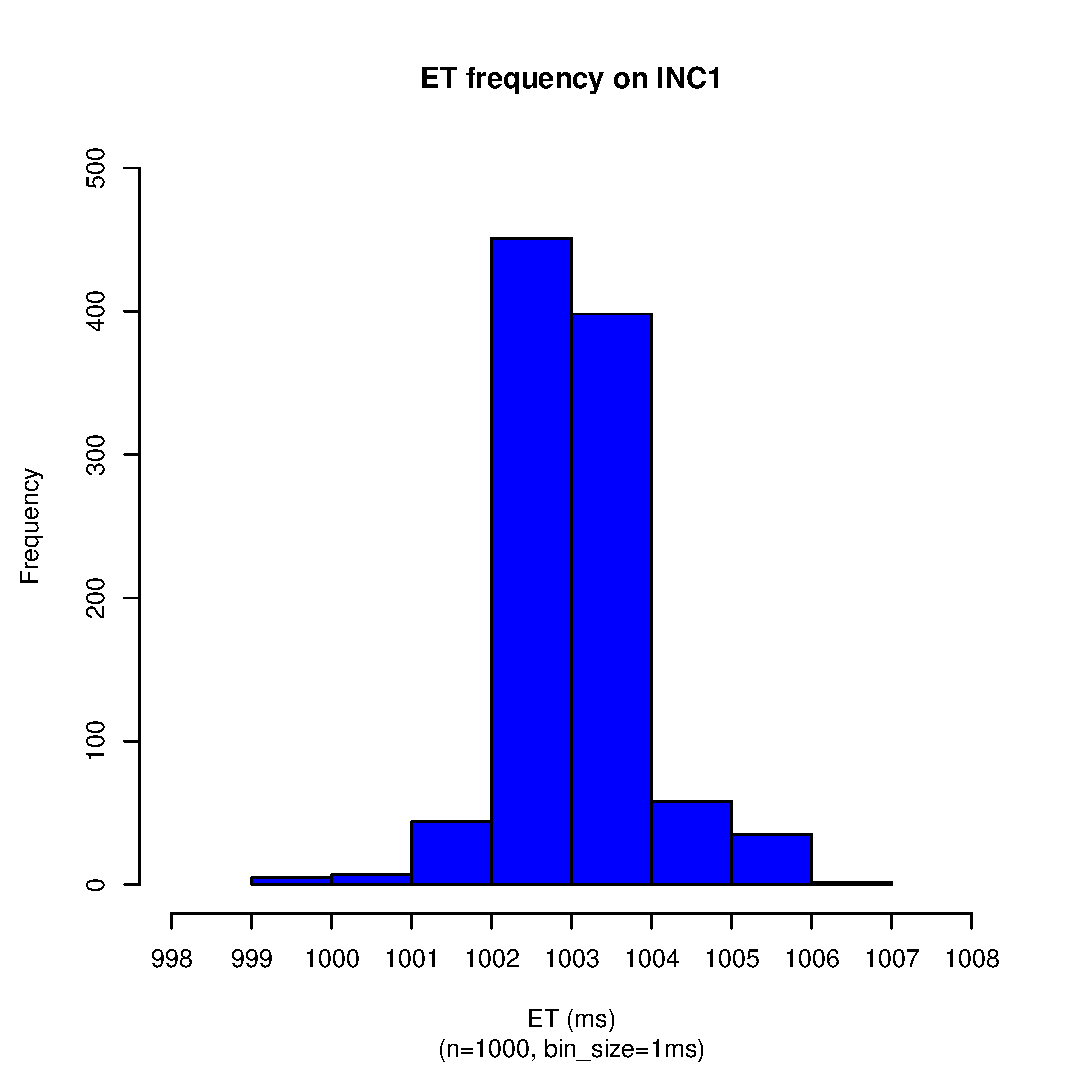
\includegraphics[scale=0.43]{1_sec_et_hist.eps}
		\label{fig:inc1_et_hist}
	}
	\subfigure[ET frequency on INC2]{
		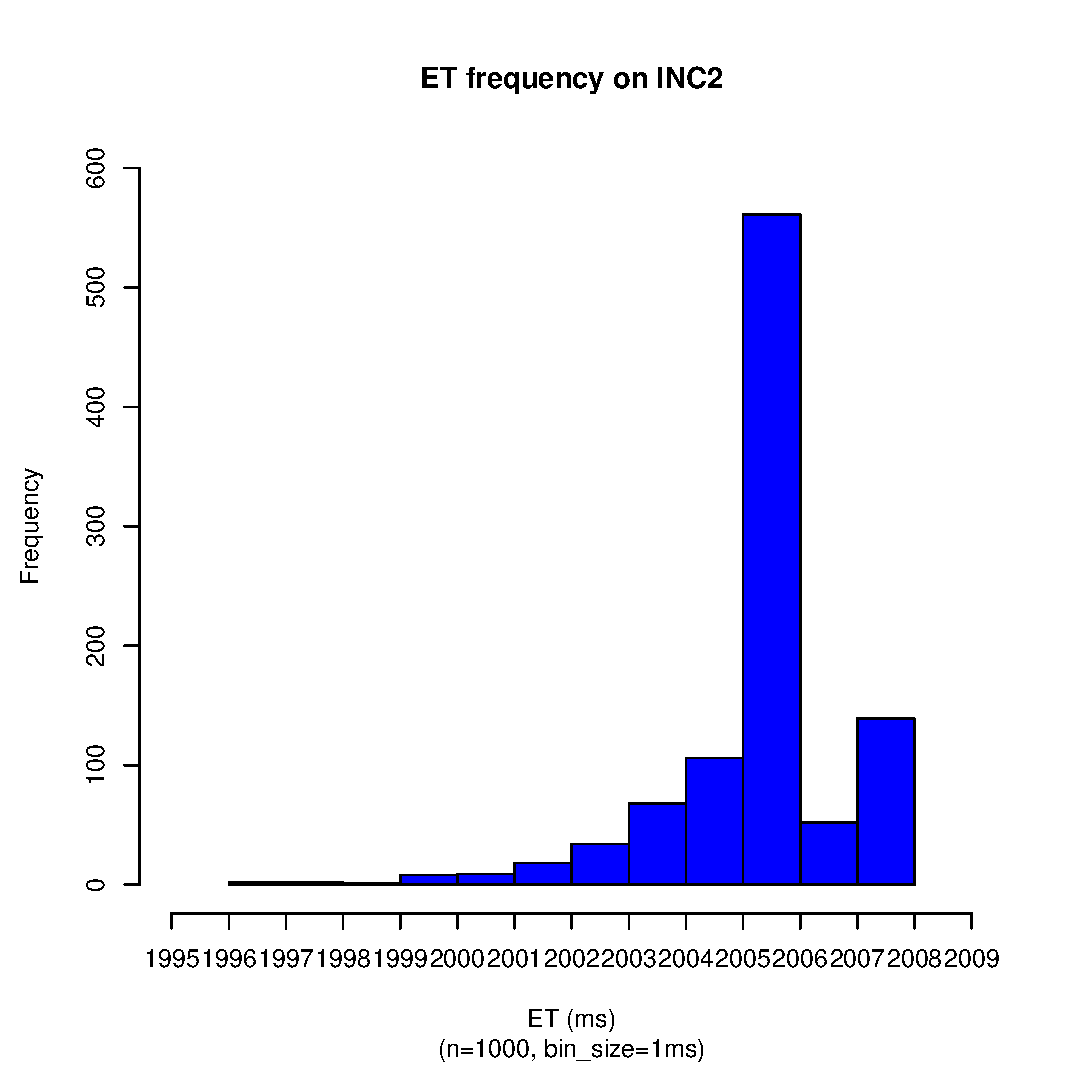
\includegraphics[scale=0.43]{2_sec_et_hist.eps}
		\label{fig:Inc2_et_hist}
	}
	\subfigure[ET frequency on INC4]{
		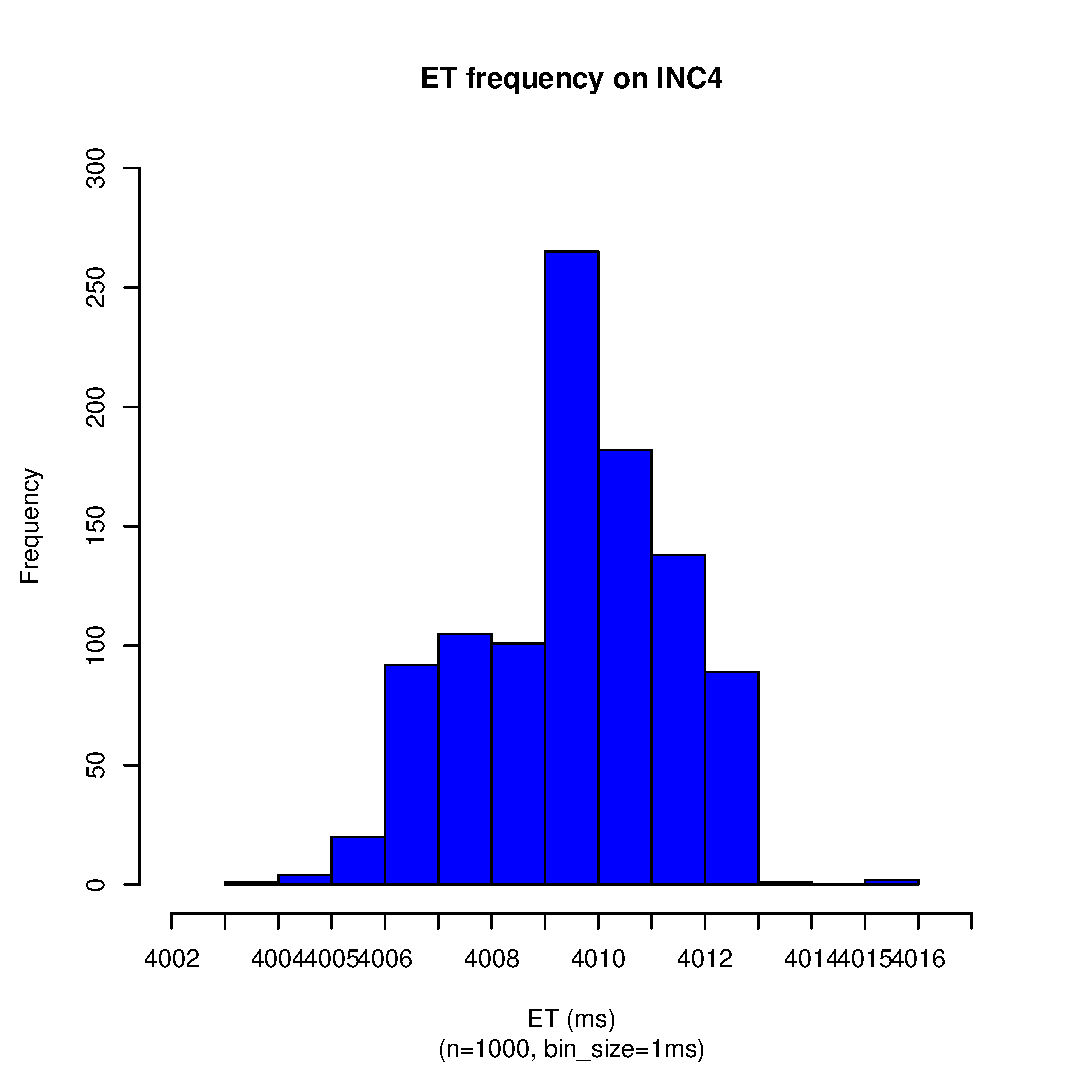
\includegraphics[scale=0.43]{4_sec_et_hist.eps}
		\label{fig:inc4_et_hist}
	}
	\subfigure[ET frequency on INC8]{
		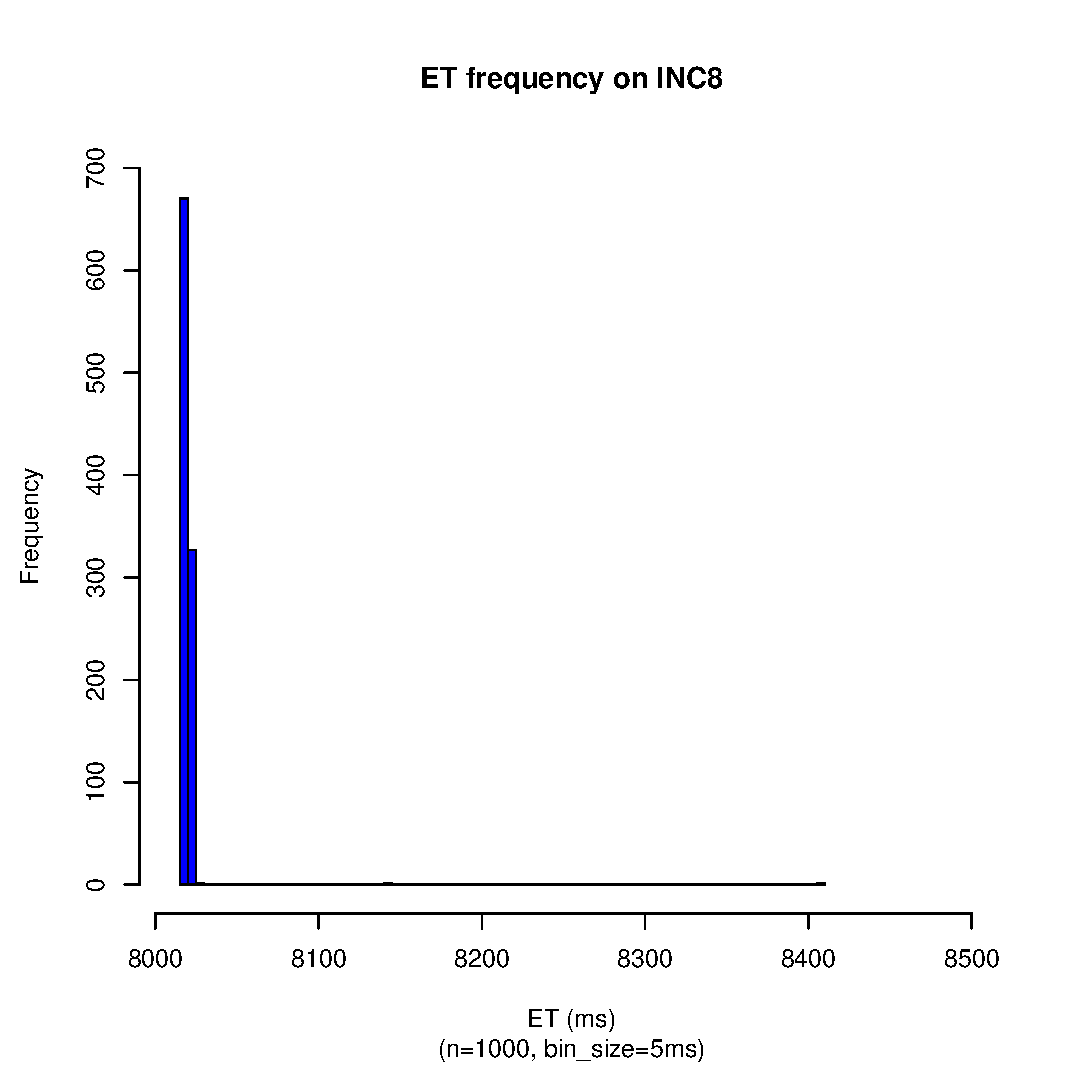
\includegraphics[scale=0.43]{8_sec_et_hist.eps}
		\label{fig:inc8_et_hist}
	}
	\caption{ET Histograms of INC1 ... INC8~\label{fig:et_hist1}}
\end{figure}

\begin{figure}[hp!]
	\centering
	\subfigure[ET frequency on INC16]{
		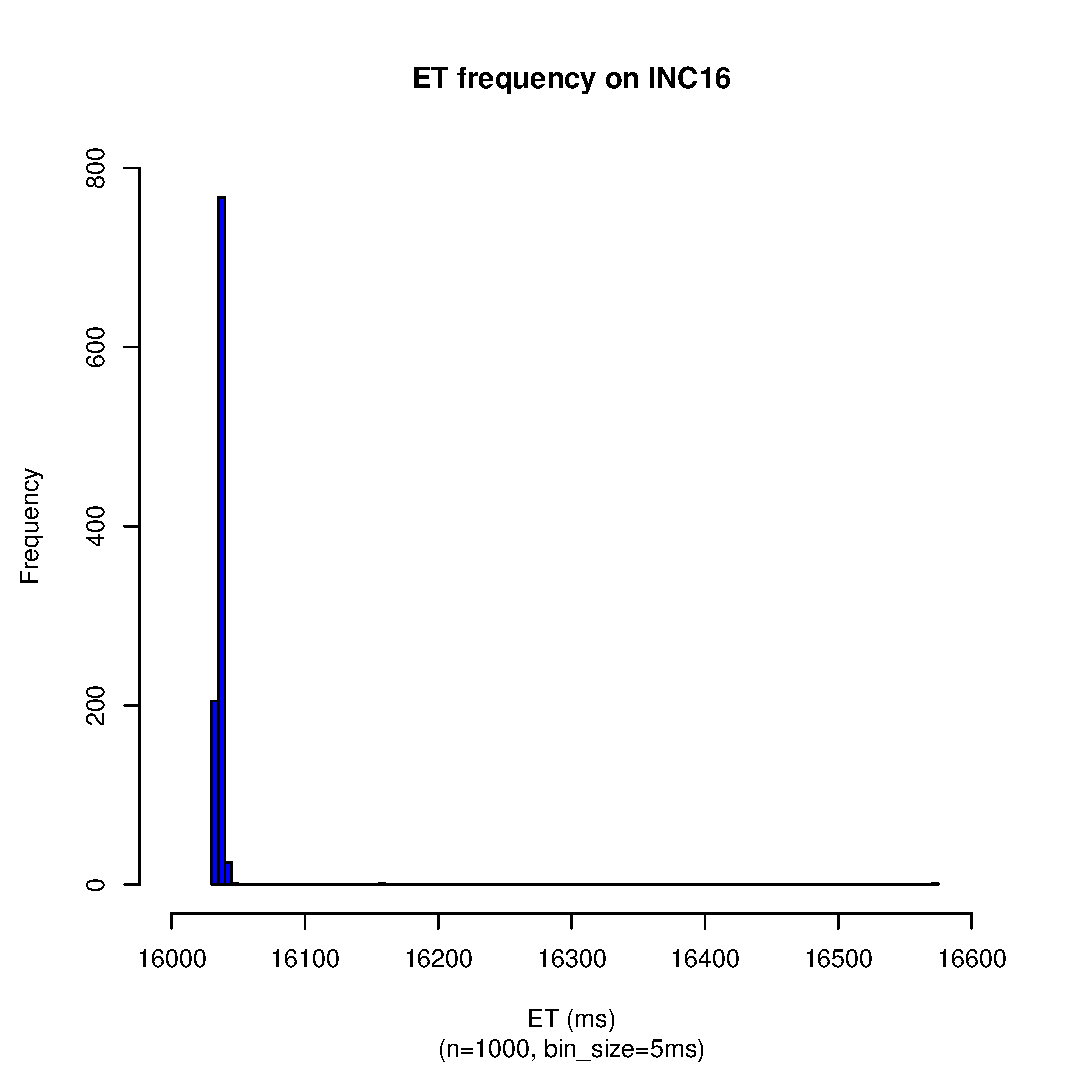
\includegraphics[scale=0.43]{16_sec_et_hist.eps}
		\label{fig:inc16_et_hist}
	}
	\subfigure[ET frequency on INC32]{
		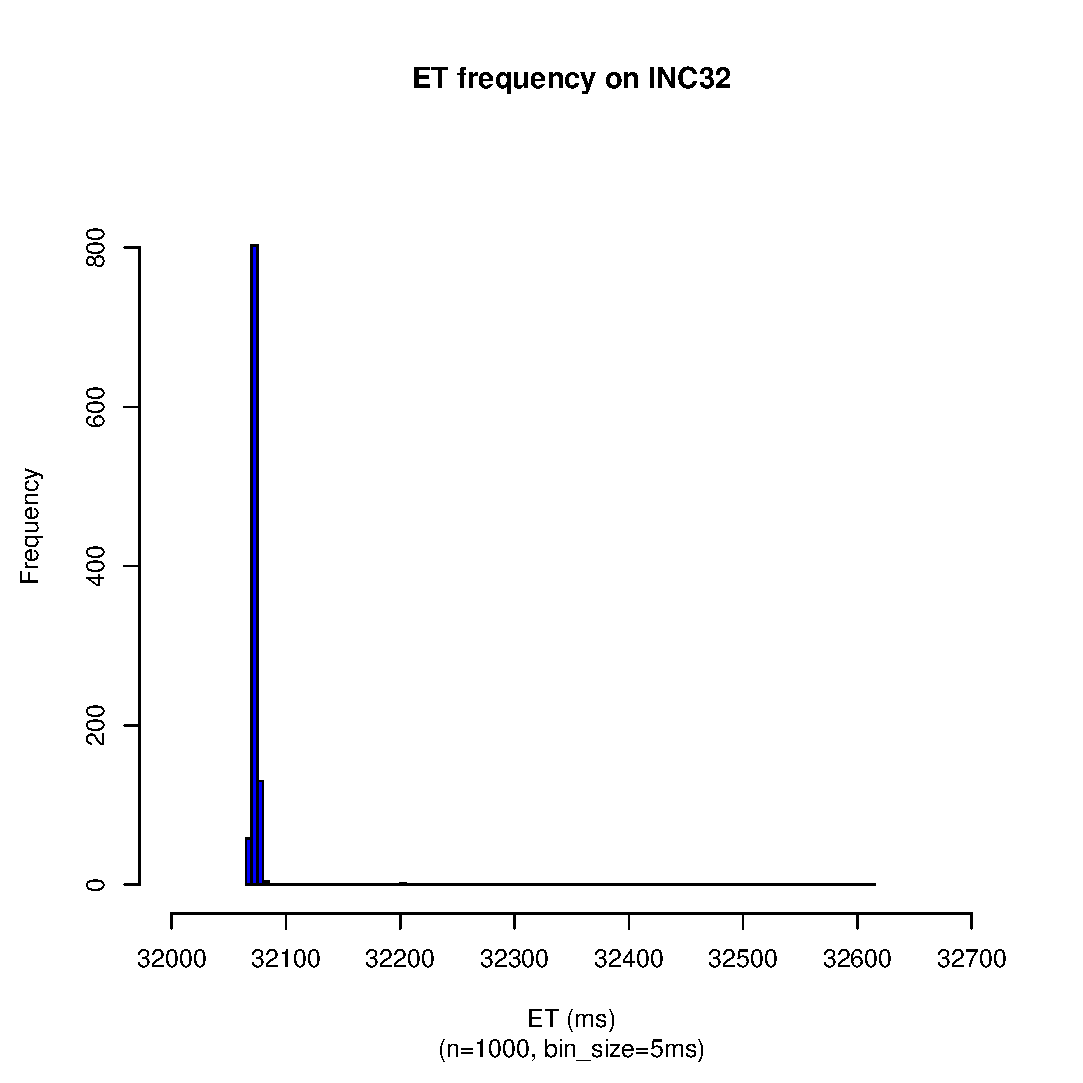
\includegraphics[scale=0.43]{32_sec_et_hist.eps}
		\label{fig:inc32_et_hist}
	}
	\subfigure[ET frequency on INC64]{
		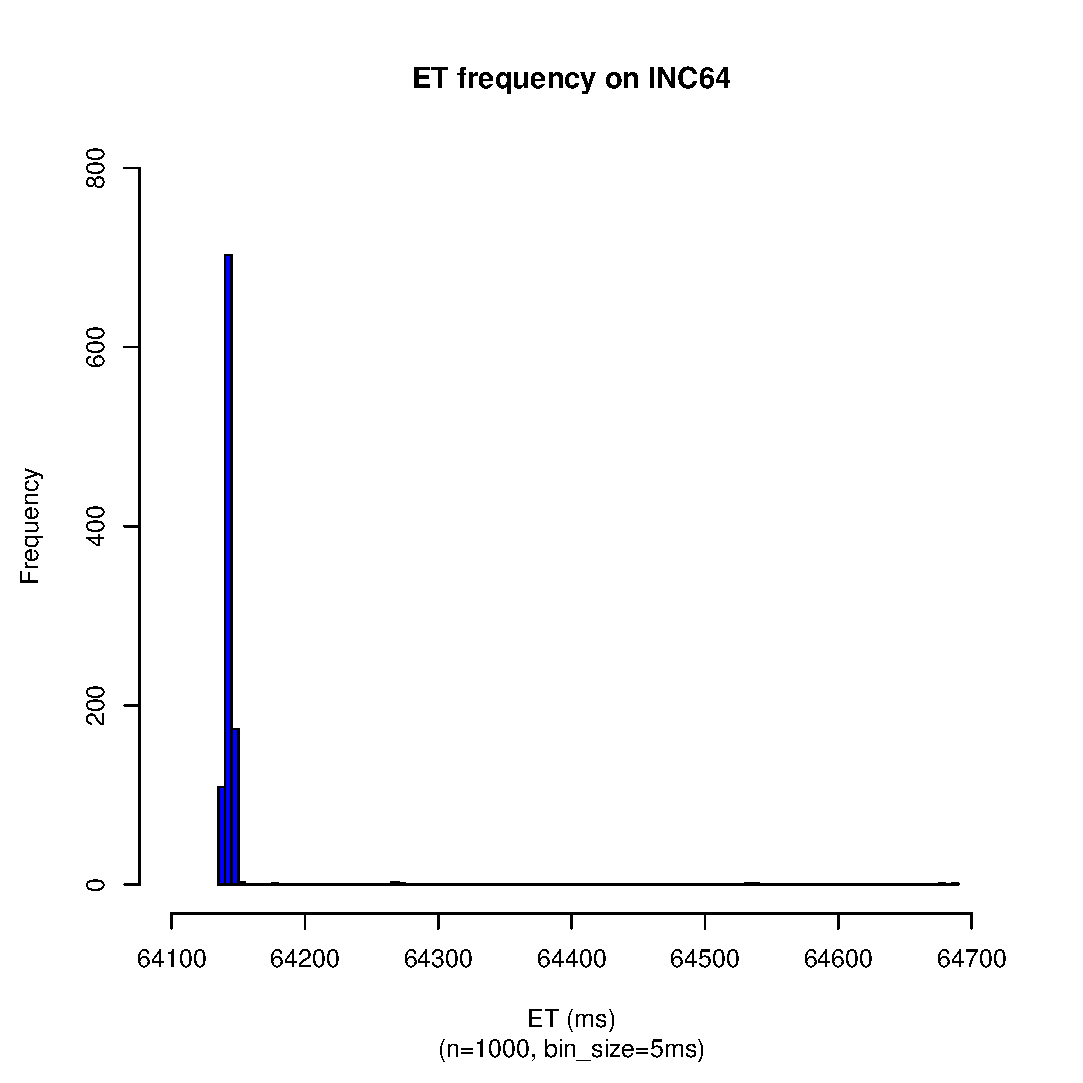
\includegraphics[scale=0.43]{64_sec_et_hist.eps}
		\label{fig:inc64_et_hist}
	}
	\caption{ET Histograms of INC16 ... INC64~\label{fig:et_hist2}}
\end{figure}

\newpage

\begin{figure}[hp!]
	\centering
	\subfigure[ET frequency on INC128]{
		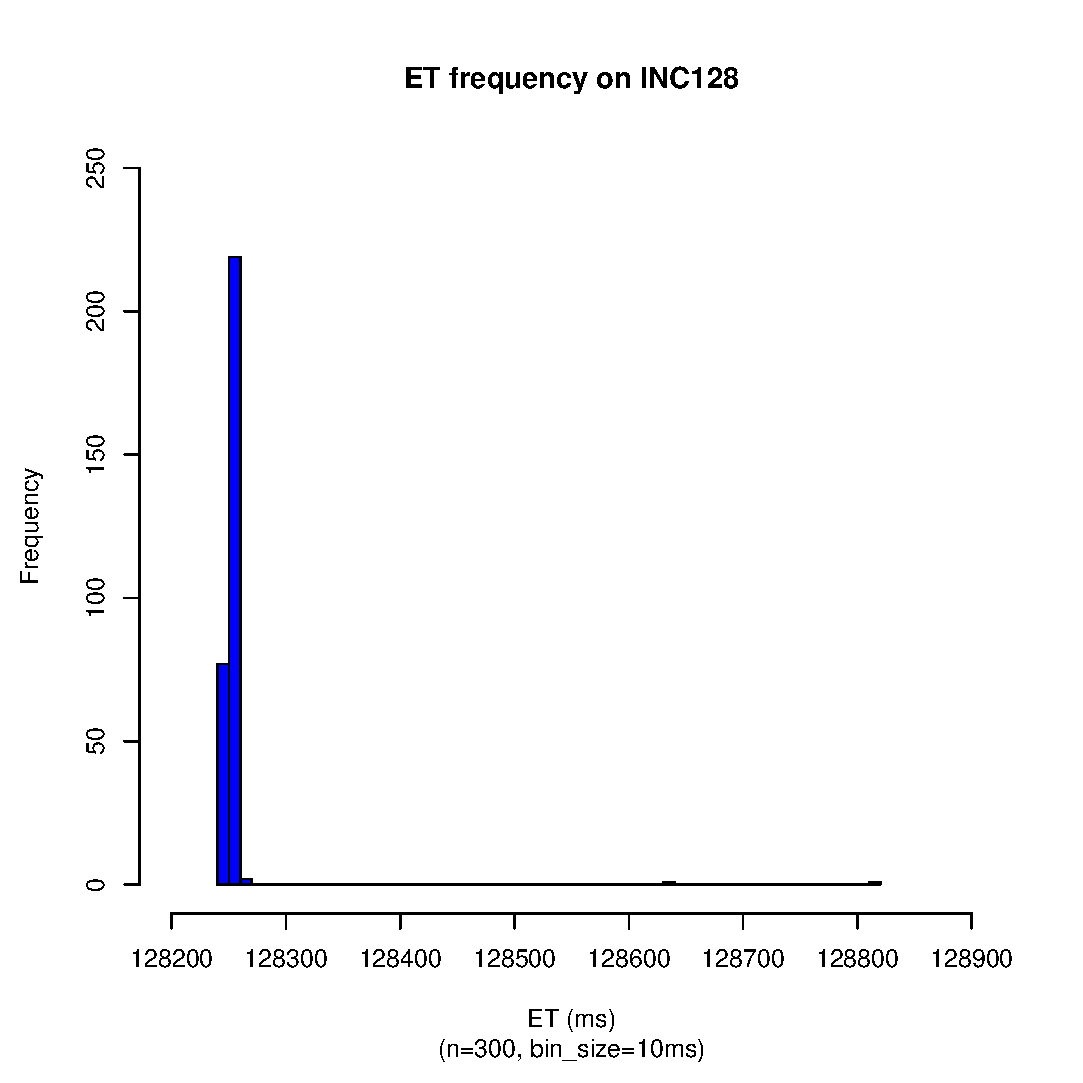
\includegraphics[scale=0.43]{128_sec_et_hist.eps}
		\label{fig:inc128_et_hist}
	}
	\subfigure[ET frequency on INC256]{
		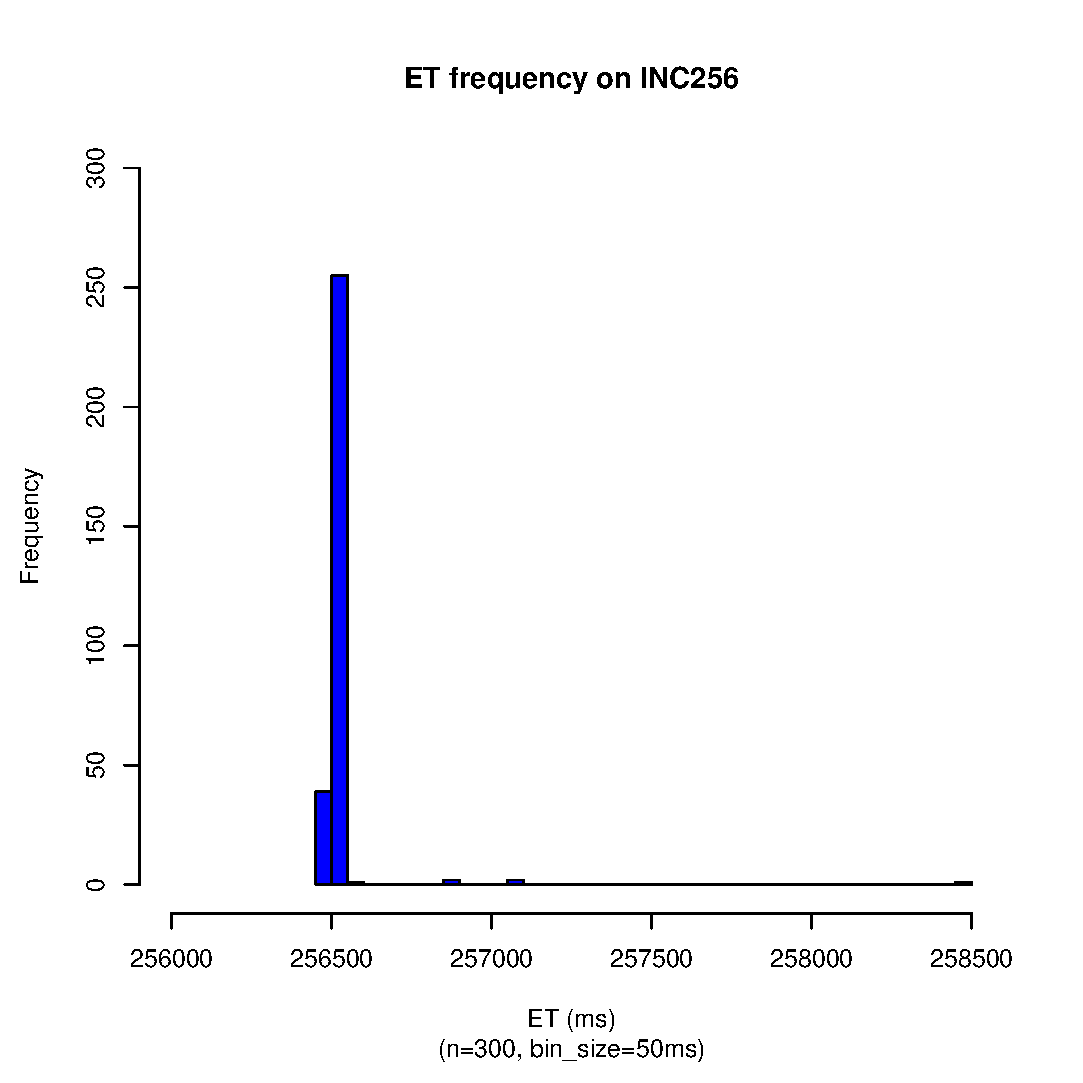
\includegraphics[scale=0.43]{256_sec_et_hist.eps}
		\label{fig:inc256_et_hist}
	}
	\subfigure[ET frequency on INC512]{
		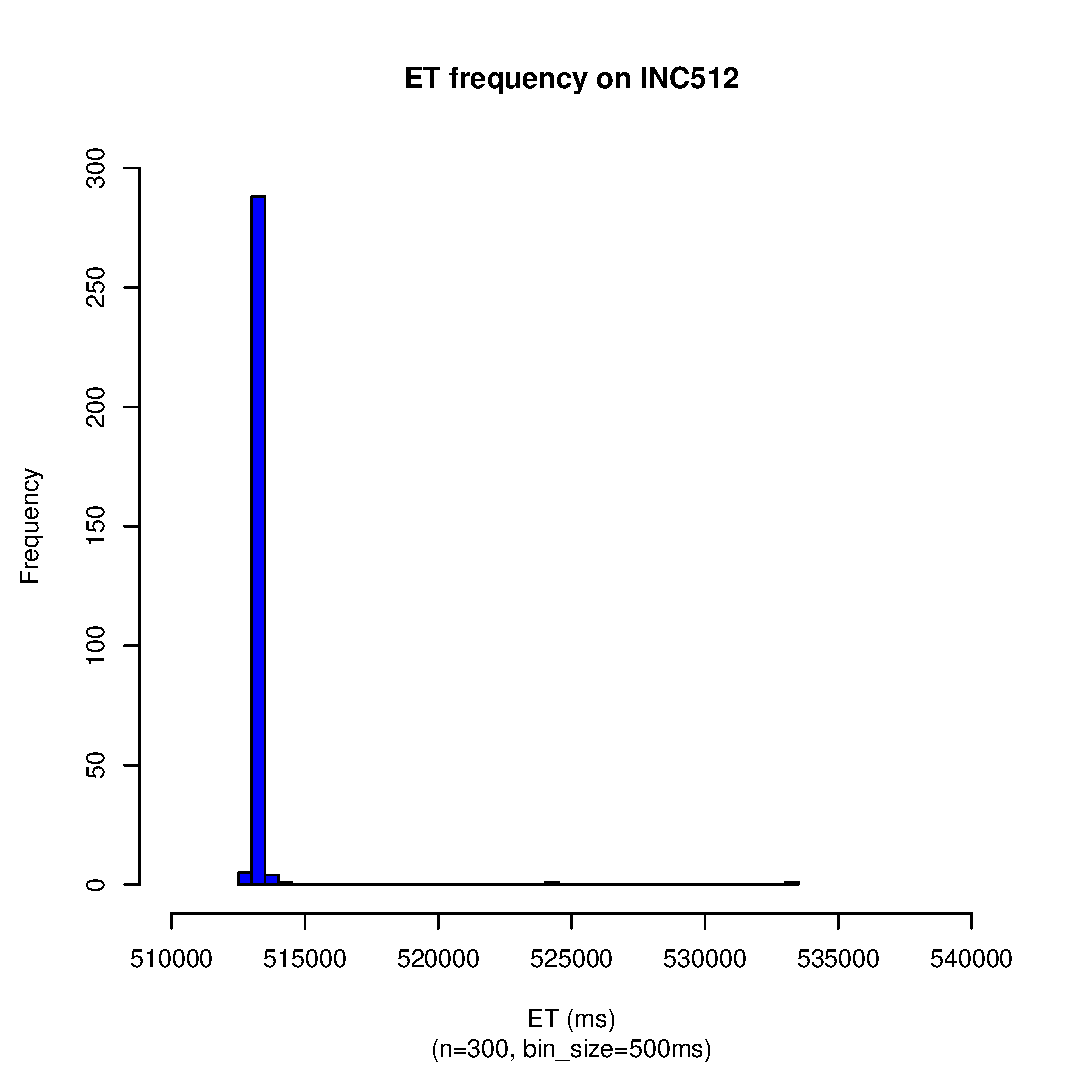
\includegraphics[scale=0.43]{512_sec_et_hist.eps}
		\label{fig:inc512_et_hist}
	}
	\subfigure[ET frequency on INC1024]{
		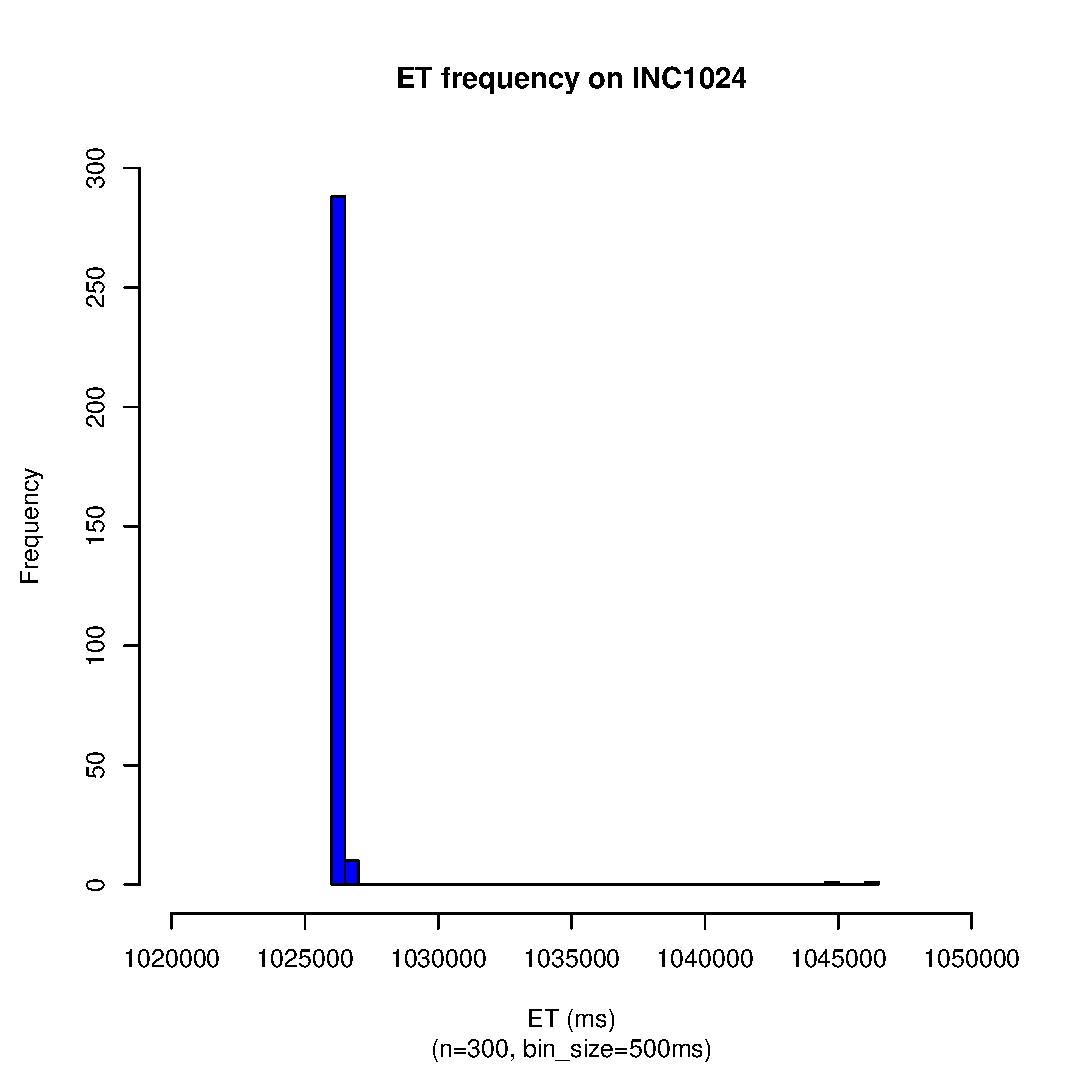
\includegraphics[scale=0.43]{1024_sec_et_hist.eps}
		\label{fig:inc1024_et_hist}
	}
	\caption{ET Histograms of INC128 ... INC1024~\label{fig:et_hist3}}
\end{figure}

\newpage

\begin{figure}[hp!]
	\centering
	\subfigure[ET frequency on INC2048]{
		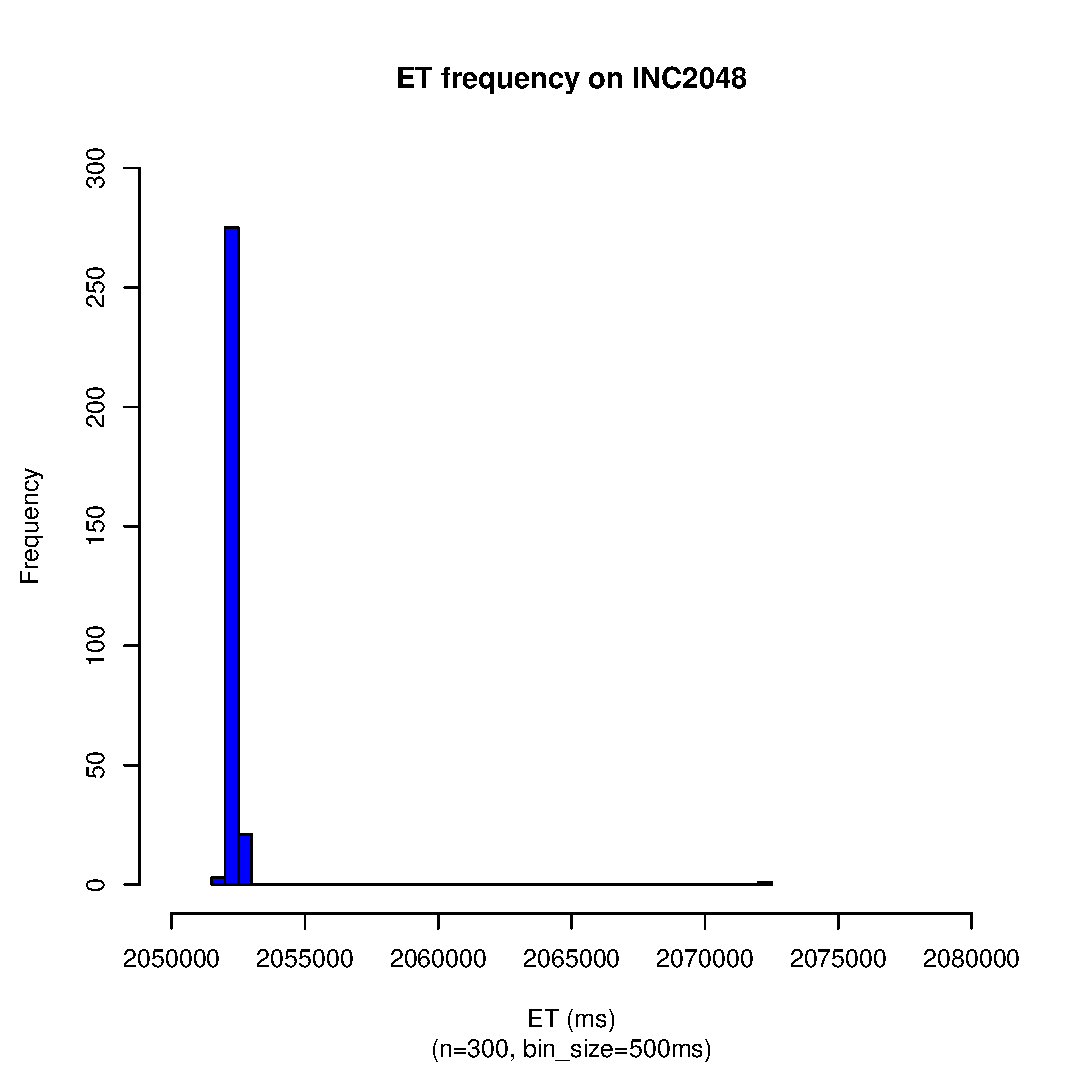
\includegraphics[scale=0.43]{2048_sec_et_hist.eps}
		\label{fig:inc2048_et_hist}
	}
	\subfigure[ET frequency on INC4096]{
		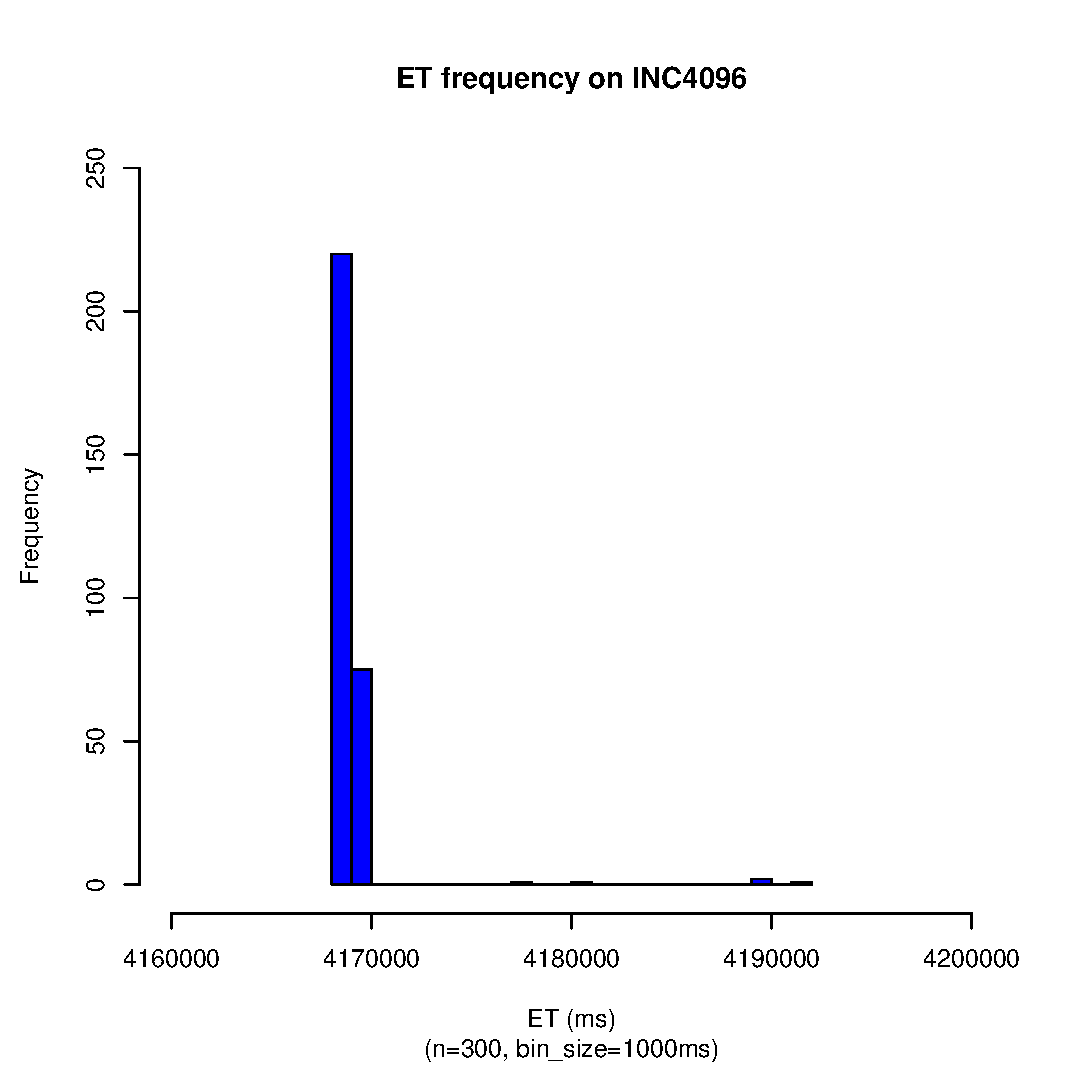
\includegraphics[scale=0.43]{4096_sec_et_hist.eps}
		\label{fig:inc4096_et_hist}
	}
	\subfigure[ET frequency on INC8192]{
		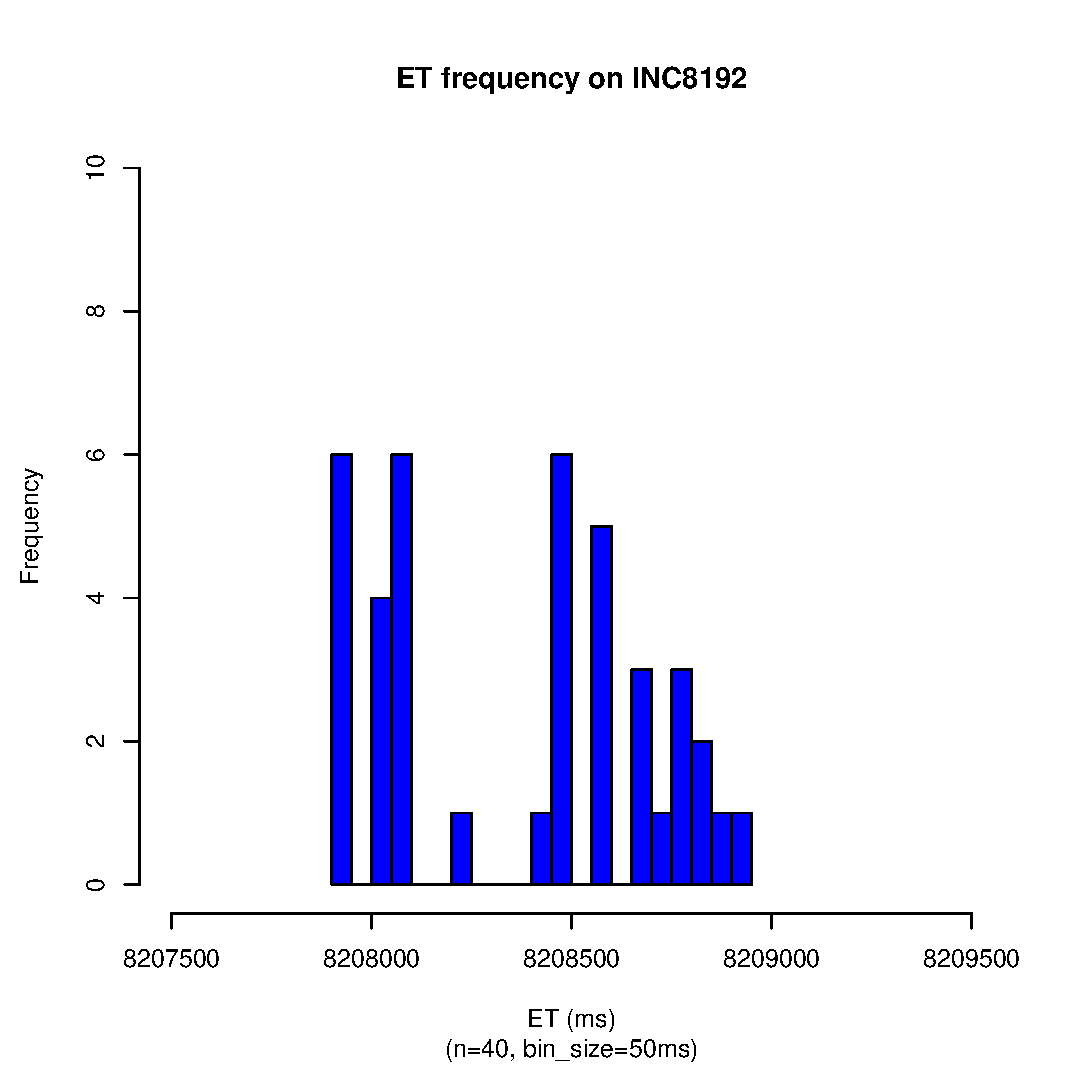
\includegraphics[scale=0.43]{8192_sec_et_hist.eps}
		\label{fig:inc8192_et_hist}
	}
	\subfigure[ET frequency on INC16384]{
		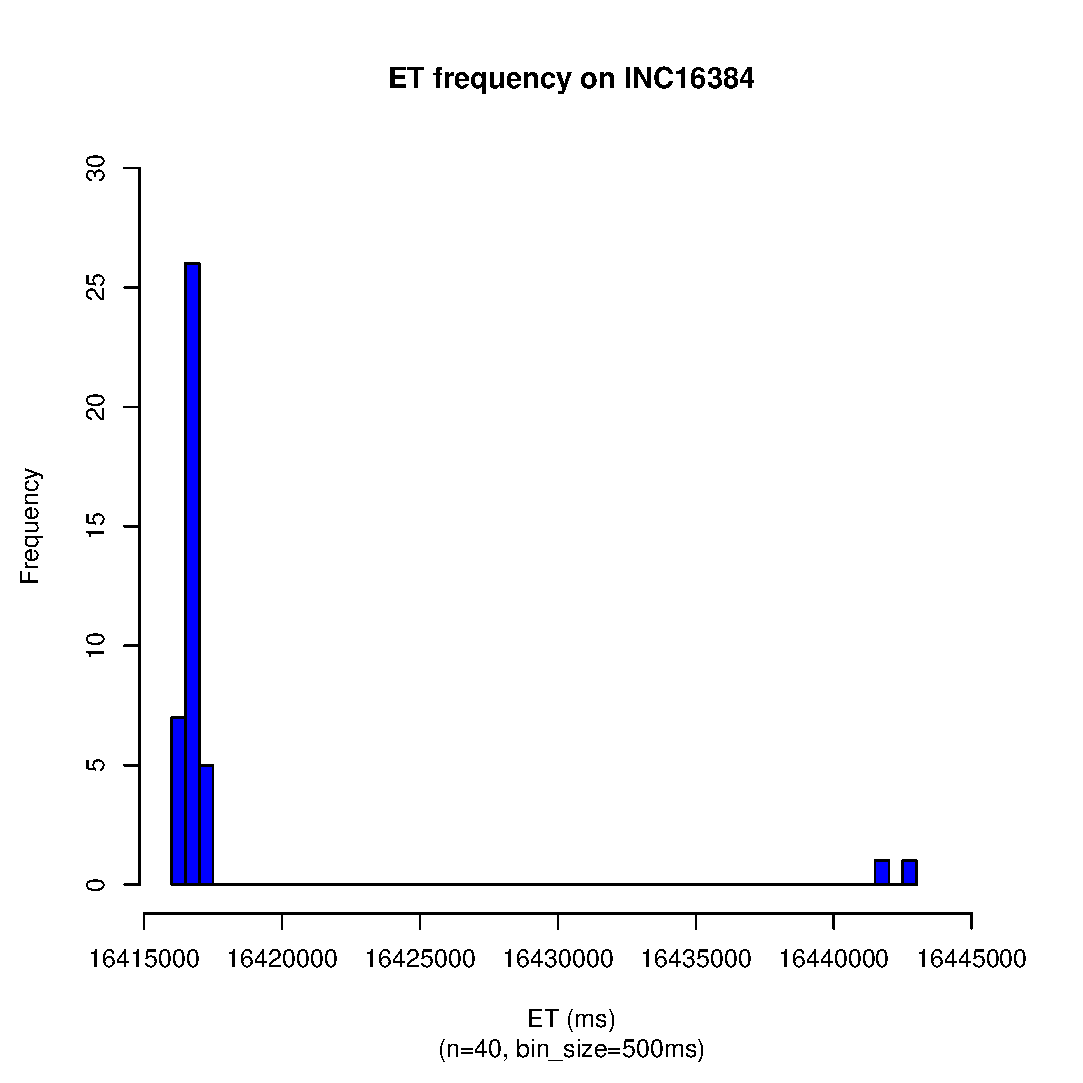
\includegraphics[scale=0.43]{16384_sec_et_hist.eps}
		\label{fig:inc16384_et_hist}
	}
	\caption{ET Histograms of INC2048 $...$ INC16384~\label{fig:et_hist4}}
\end{figure}

\newpage

\subsection{PT}

\begin{figure}[hp!]
	\centering
	\subfigure[PT frequency on INC1]{
		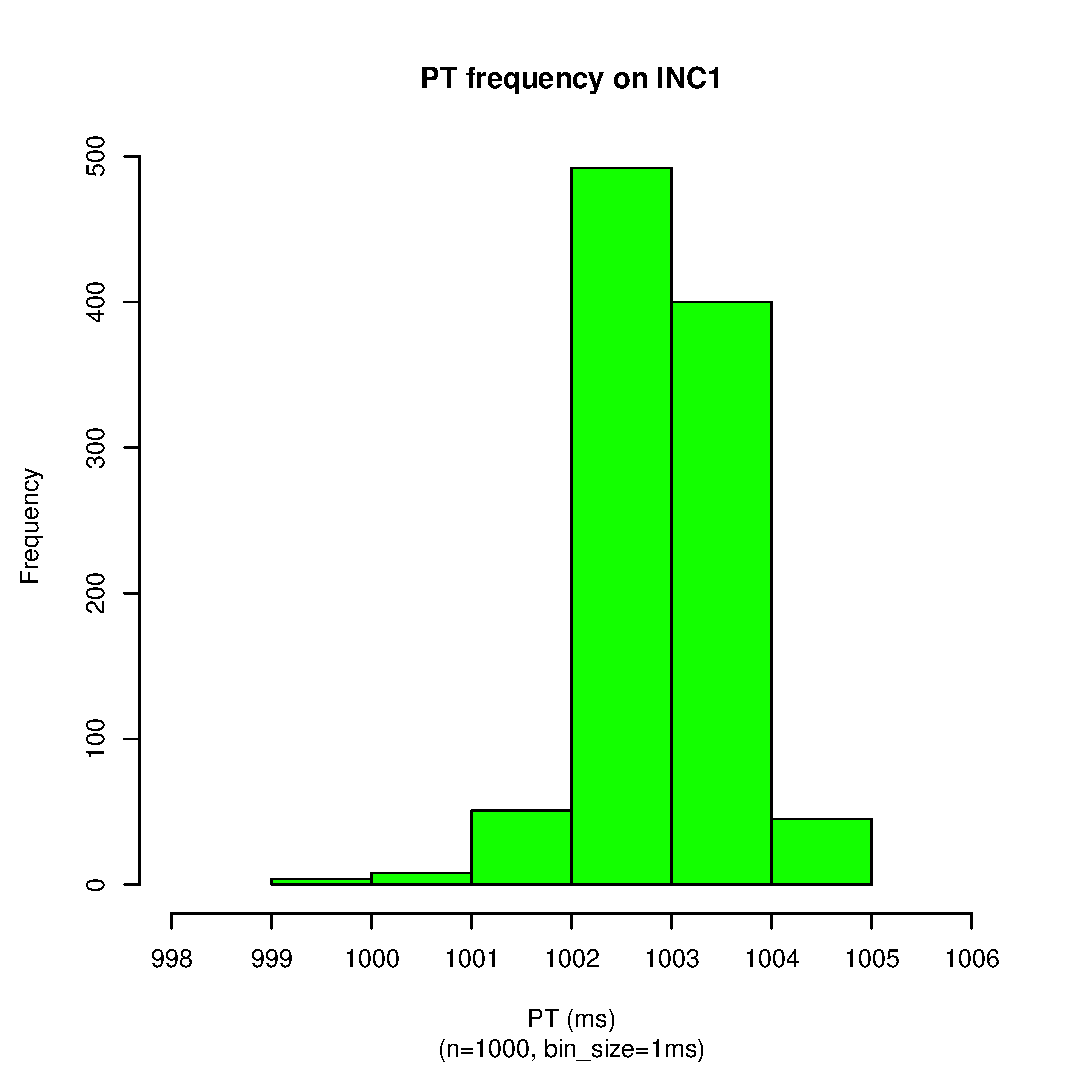
\includegraphics[scale=0.43]{1_sec_pt_hist.eps}
		\label{fig:inc1_hist}
	}
	\subfigure[PT frequency on INC2]{
		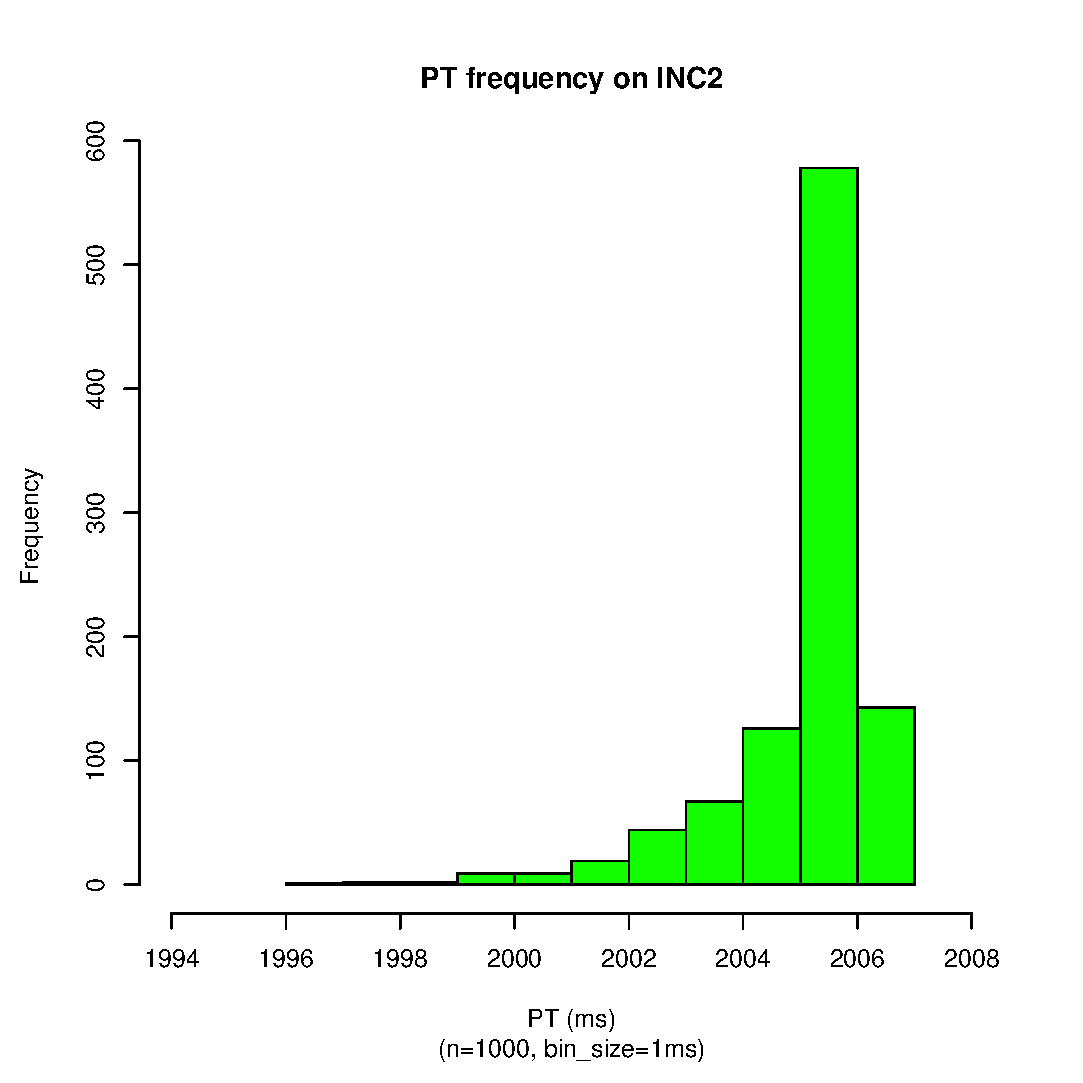
\includegraphics[scale=0.43]{2_sec_pt_hist.eps}
		\label{fig:inc2_hist}
	}
	\subfigure[PT frequency on INC4]{
		\includegraphics[scale=0.43]{4_sec_pt_hist.eps}
		\label{fig:inc4_hist}
	}
	\subfigure[PT frequency on INC8]{
		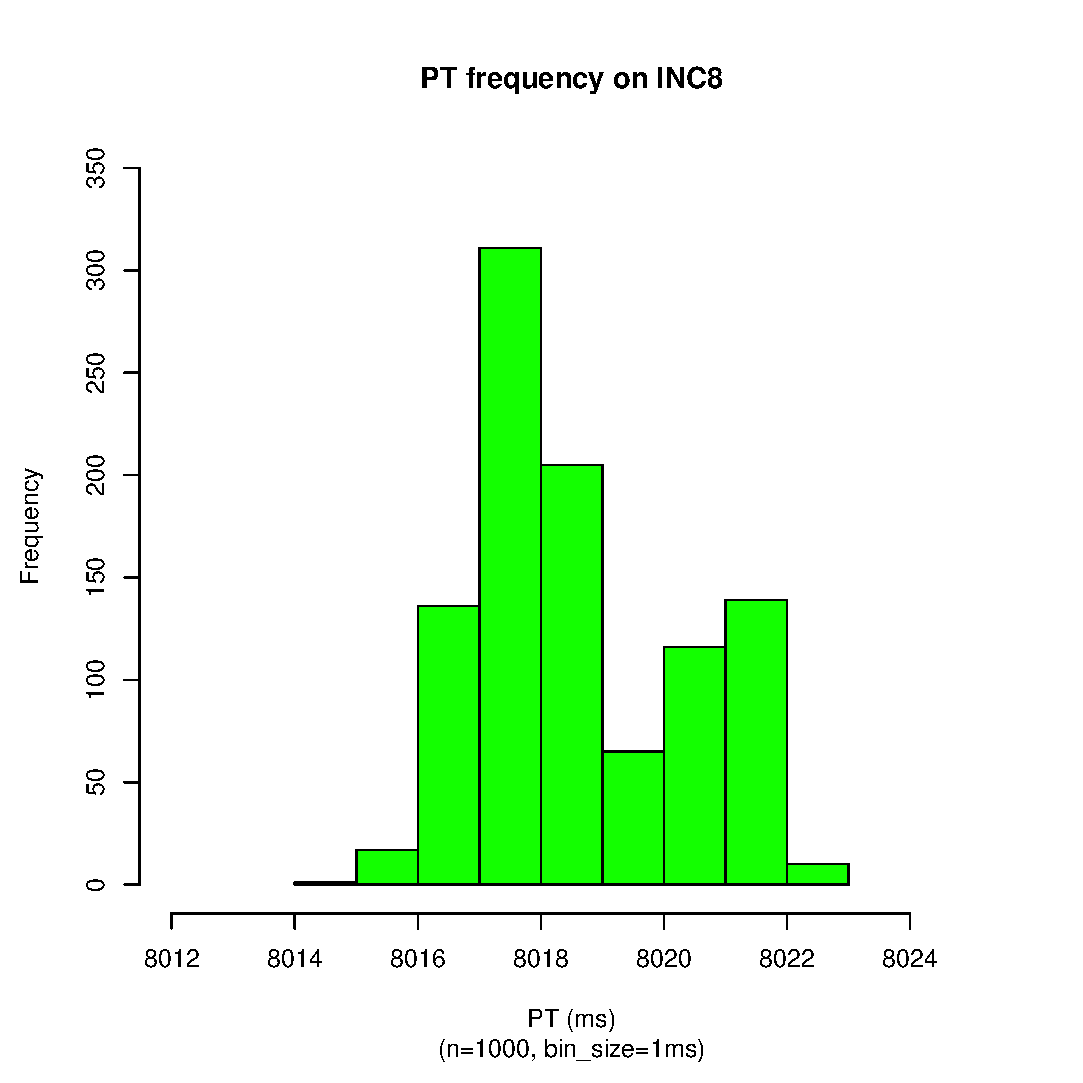
\includegraphics[scale=0.43]{8_sec_pt_hist.eps}
		\label{fig:inc8_hist}
	}
	\caption{PT Histograms of INC1 ... INC8~\label{fig:pt_hist1}}
\end{figure}

\begin{figure}[hp!]
	\centering
	\subfigure[PT frequency on INC16]{
		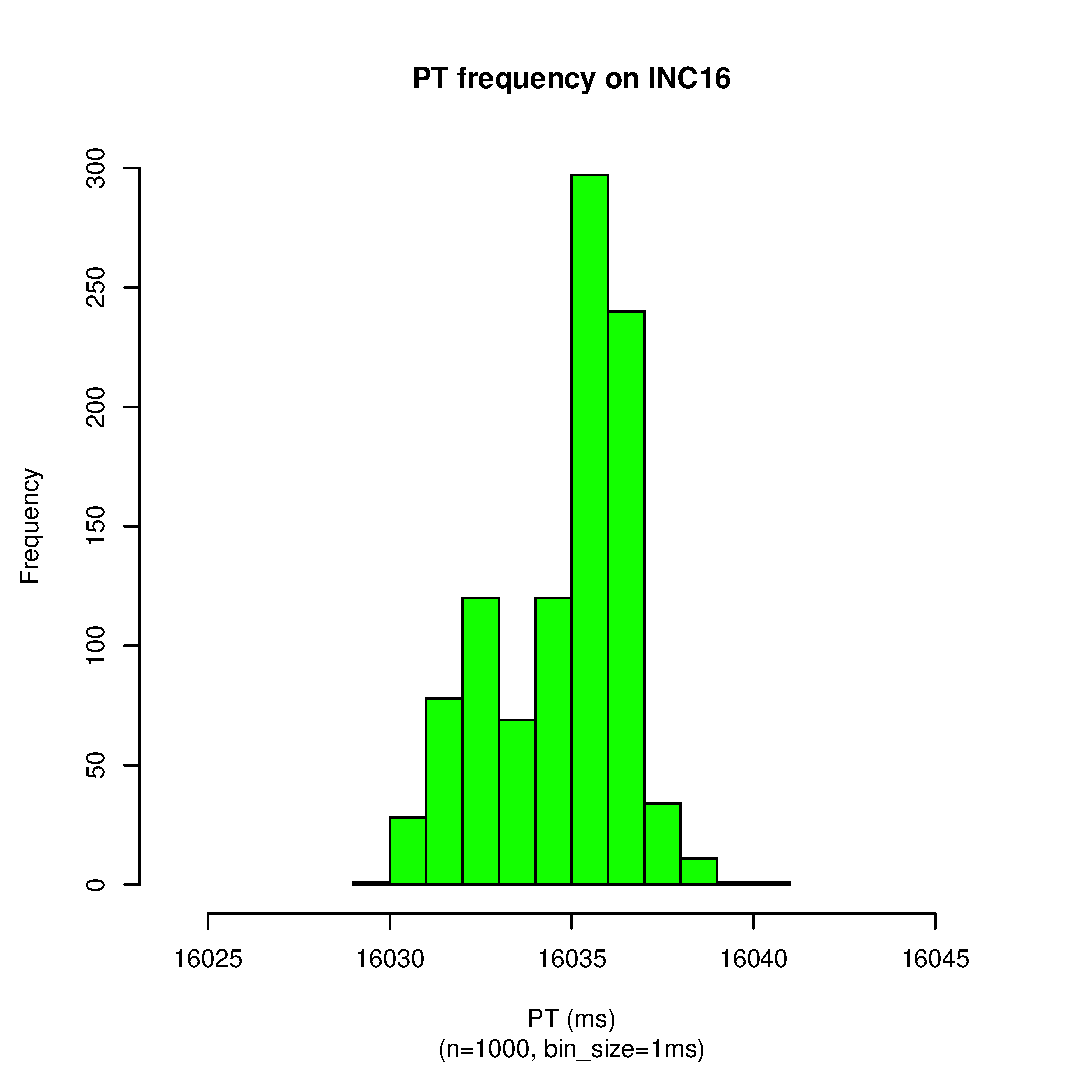
\includegraphics[scale=0.43]{16_sec_pt_hist.eps}
		\label{fig:put16_hist}
	}
	\subfigure[PT frequency on INC32]{
		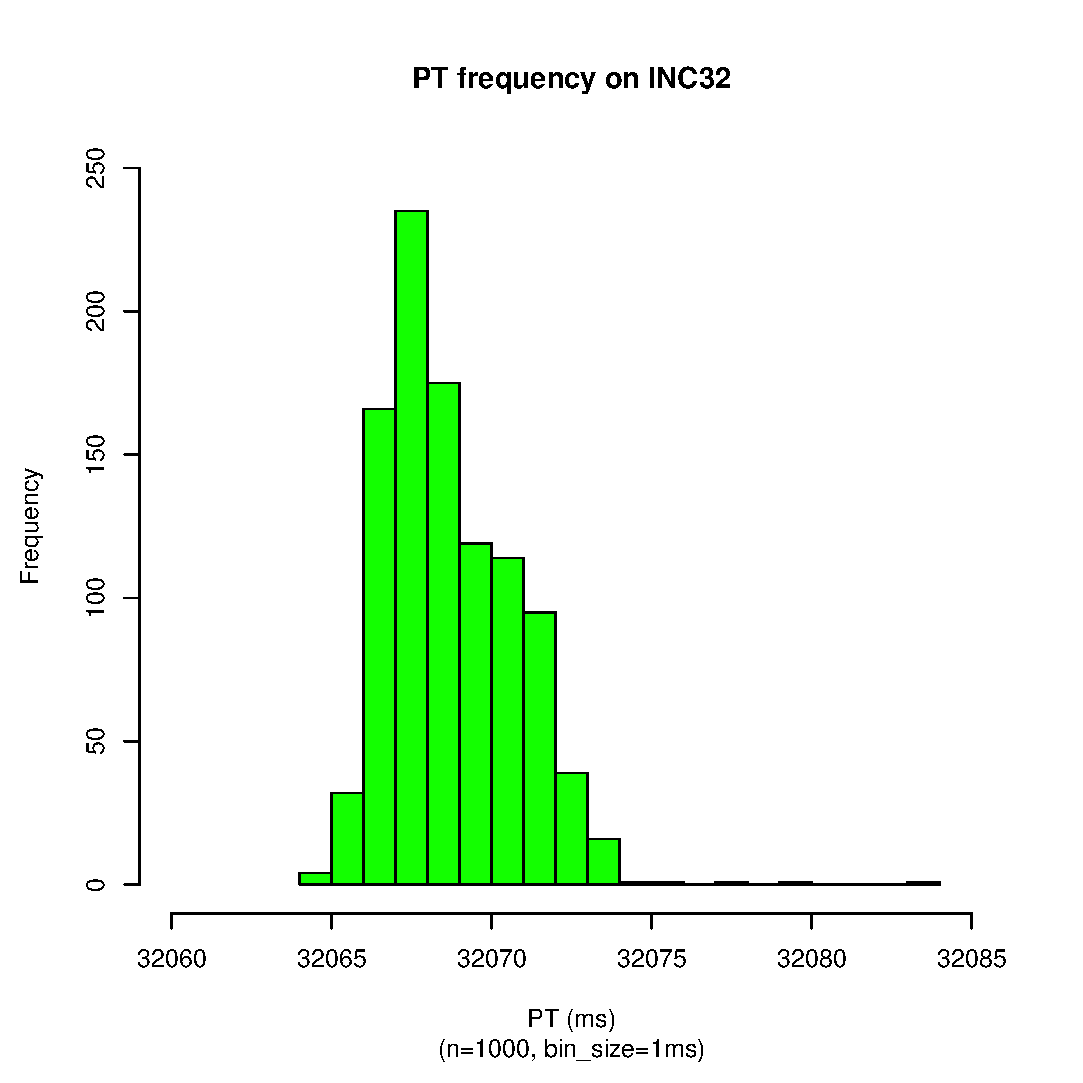
\includegraphics[scale=0.43]{32_sec_pt_hist.eps}
		\label{fig:put32_hist}
	}
	\subfigure[PT frequency on INC64]{
		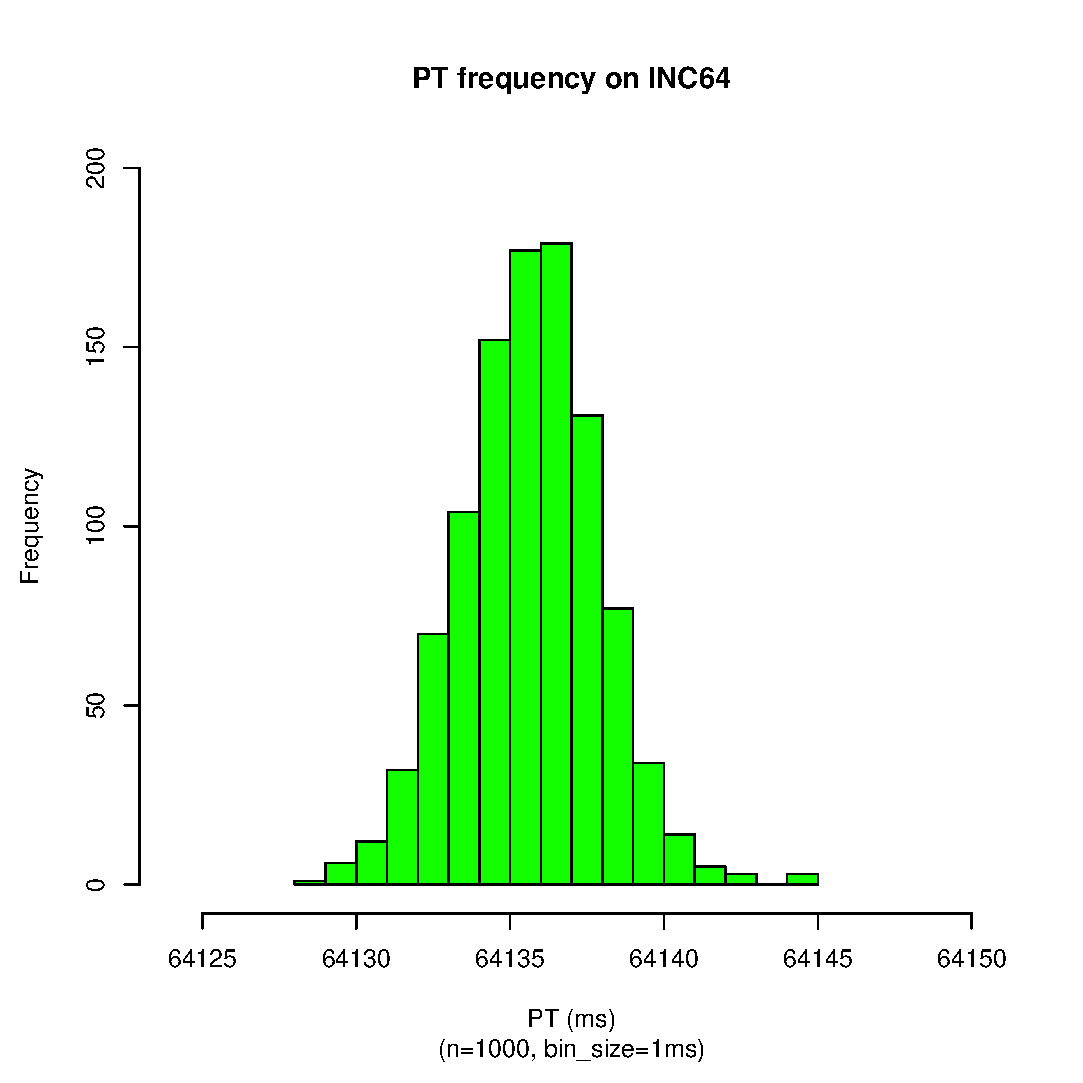
\includegraphics[scale=0.43]{64_sec_pt_hist.eps}
		\label{fig:put64_hist}
	}
	\caption{PT Histograms of INC16 ... INC64~\label{fig:pt_hist2}}
\end{figure}

\newpage

\begin{figure}[hp!]
	\centering
	\subfigure[PT frequency on INC128]{
		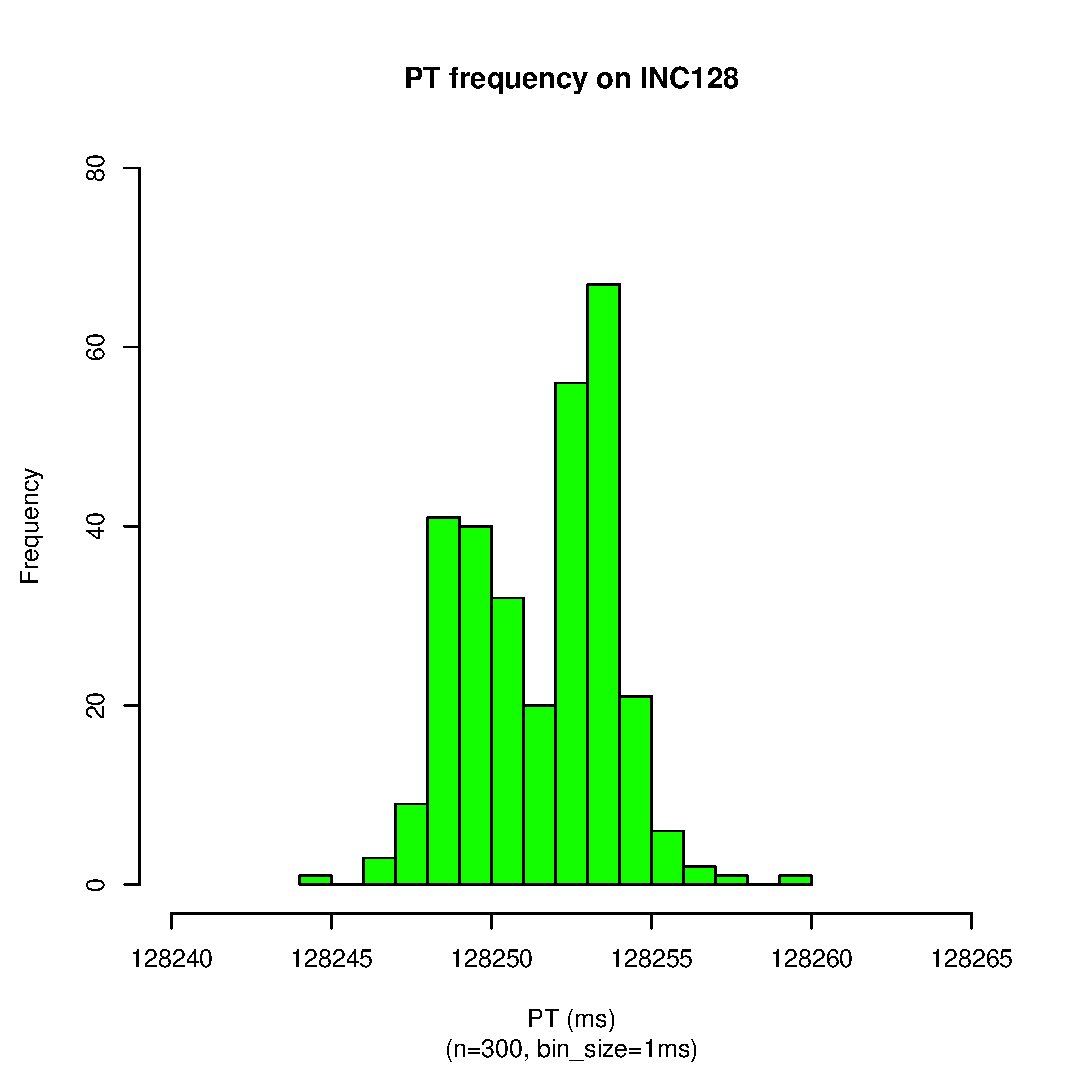
\includegraphics[scale=0.43]{128_sec_pt_hist.eps}
		\label{fig:put128_hist}
	}
	\subfigure[PT frequency on INC256]{
		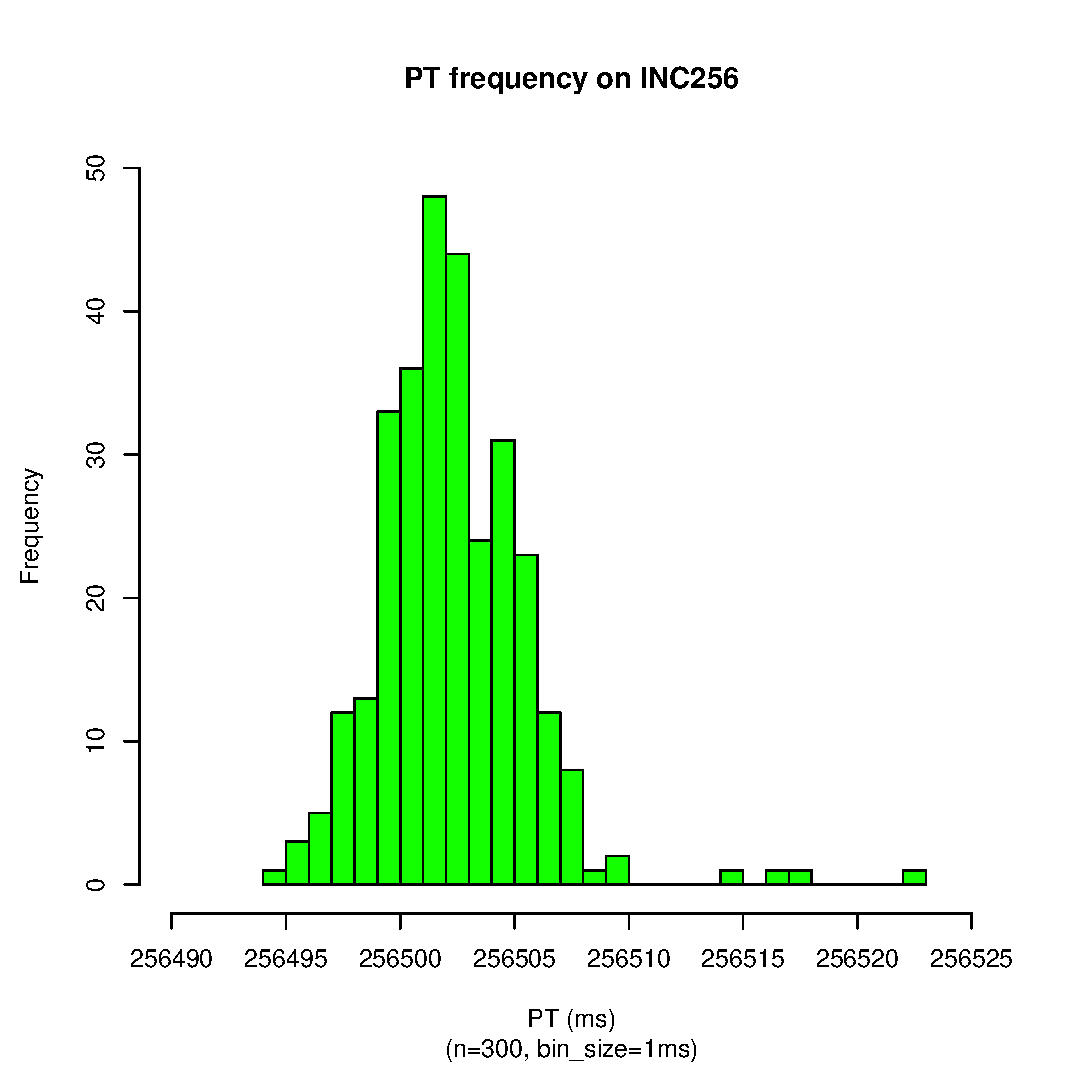
\includegraphics[scale=0.43]{256_sec_pt_hist.eps}
		\label{fig:put256_hist}
	}
	\subfigure[PT frequency on INC512]{
		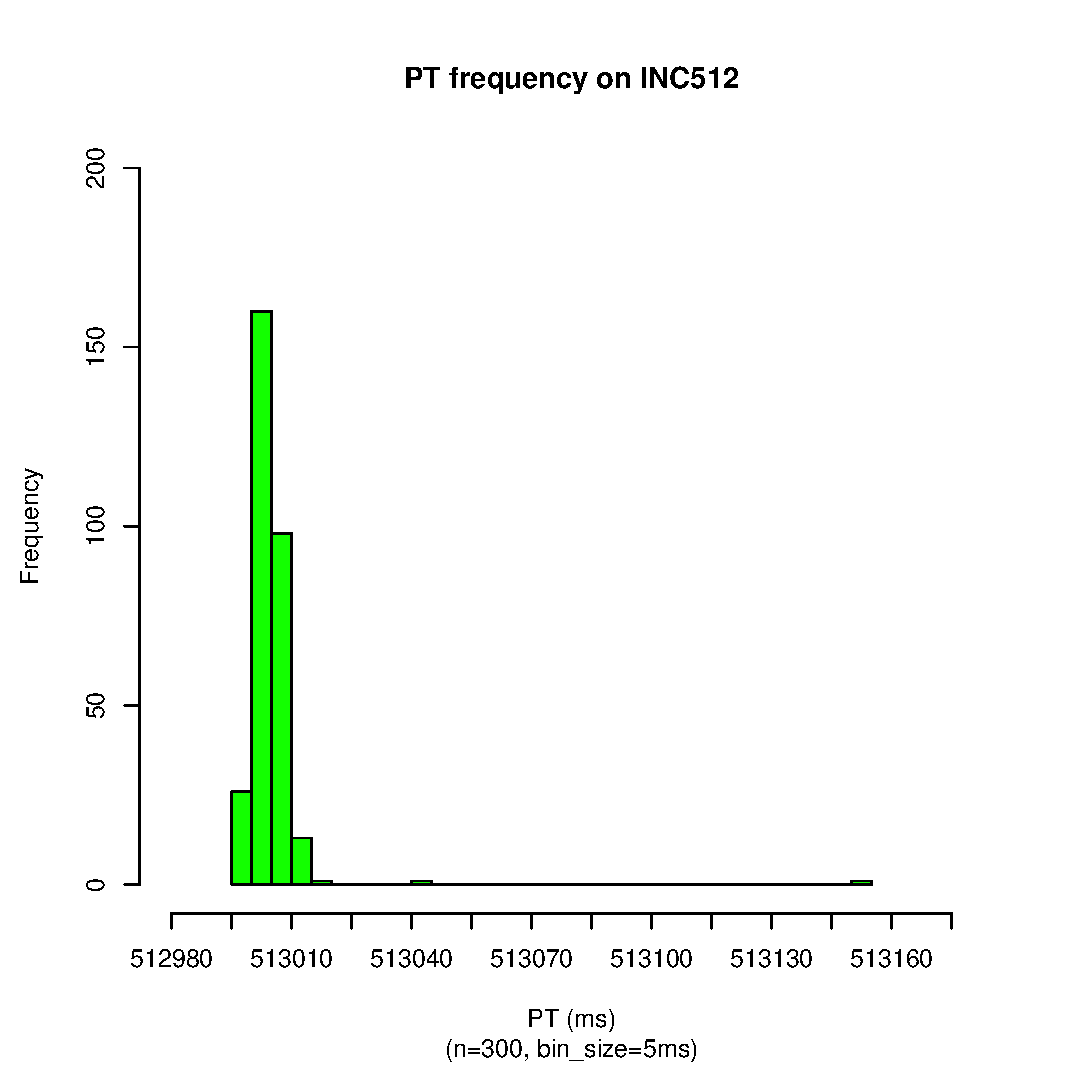
\includegraphics[scale=0.43]{512_sec_pt_hist.eps}
		\label{fig:put512_hist}
	}
	\subfigure[PT frequency on INC1024]{
		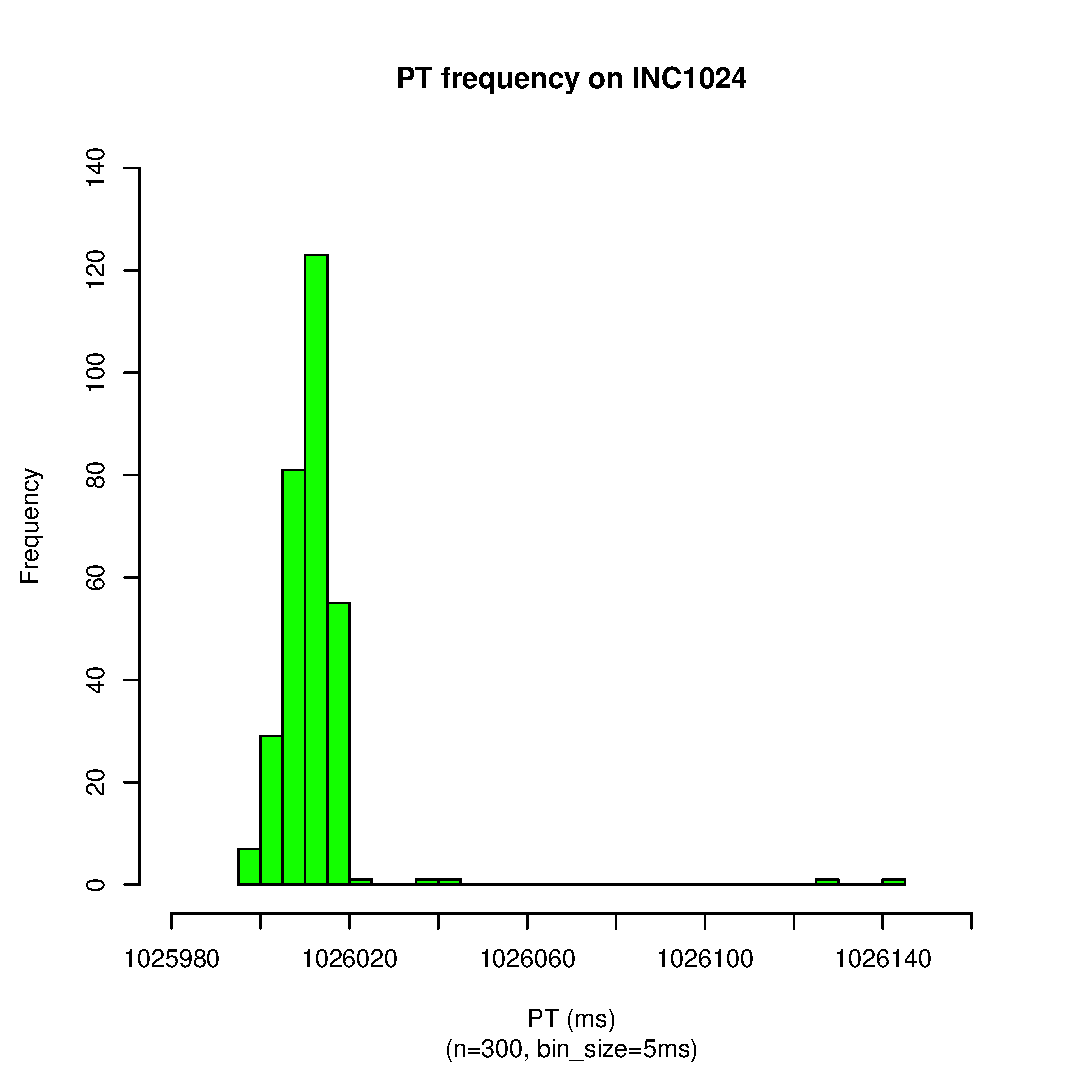
\includegraphics[scale=0.43]{1024_sec_pt_hist.eps}
		\label{fig:put1024_hist}
	}
	\caption{PT Histograms of INC128 ... INC1024~\label{fig:pt_hist3}}
\end{figure}

\newpage

\begin{figure}[hp!]
	\centering
	\subfigure[PT frequency on INC2048]{
		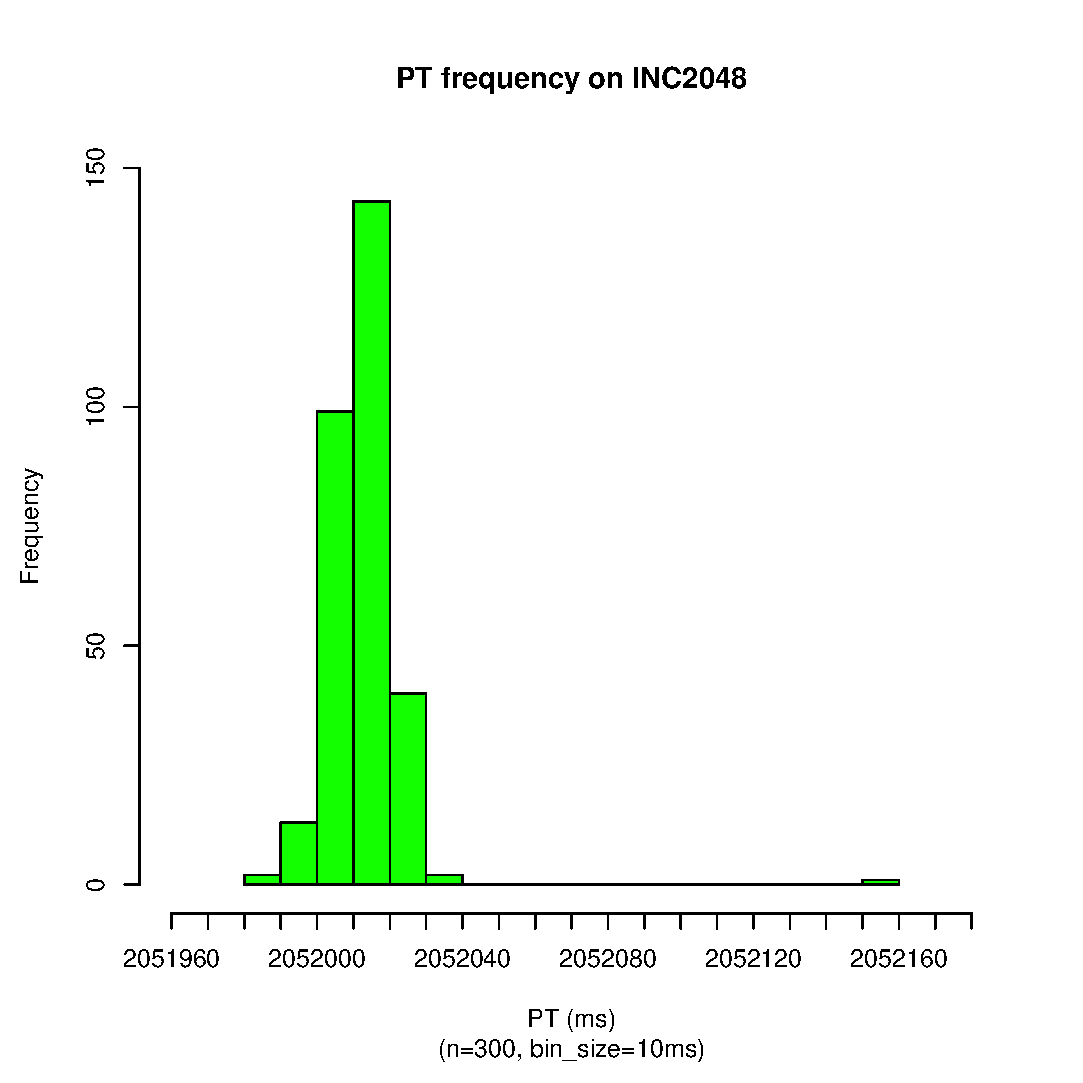
\includegraphics[scale=0.43]{2048_sec_pt_hist.eps}
		\label{fig:put2048_hist}
	}
	\subfigure[PT frequency on INC4096]{
		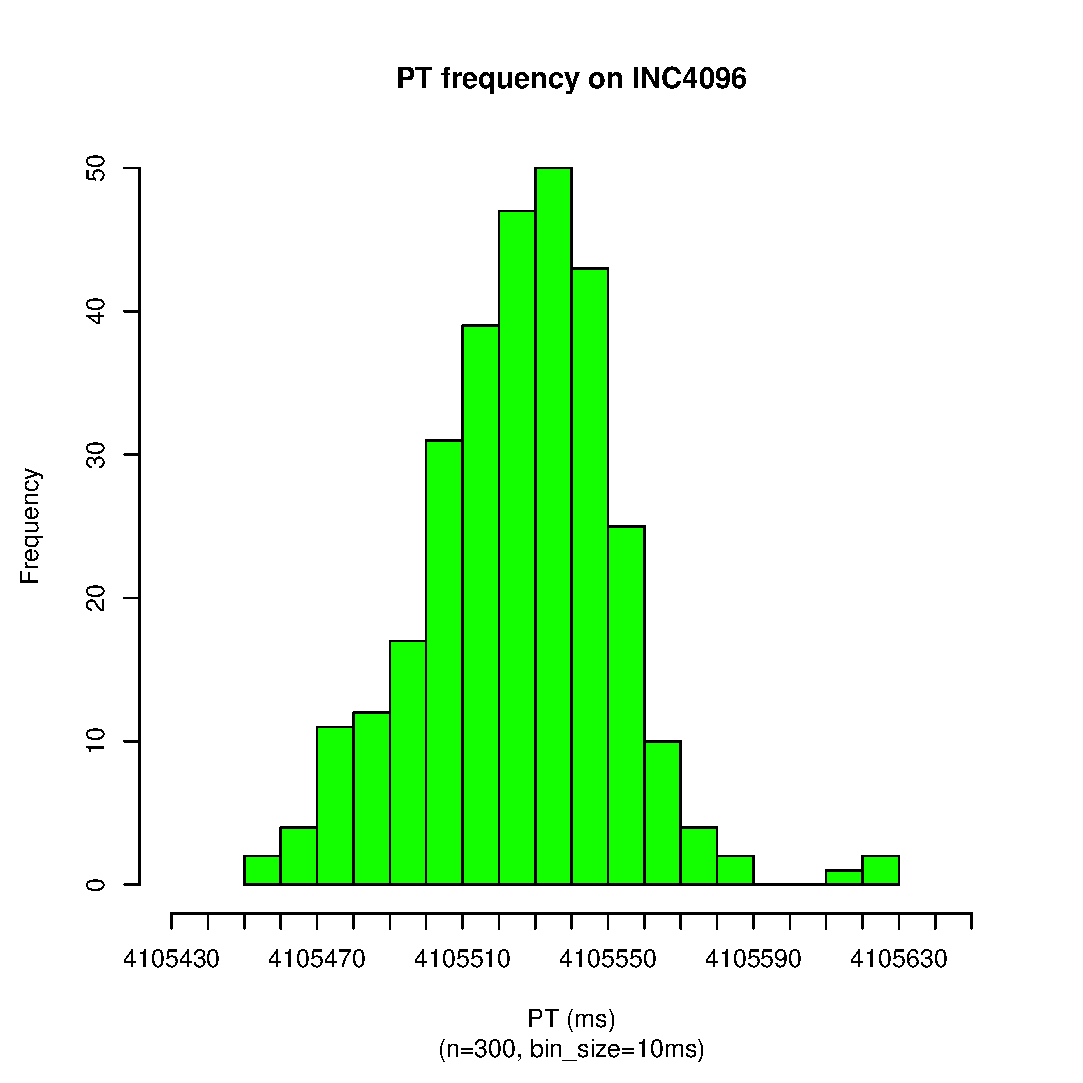
\includegraphics[scale=0.43]{4096_sec_pt_hist.eps}
		\label{fig:put4096_hist}
	}
	\subfigure[PT frequency on INC8192]{
		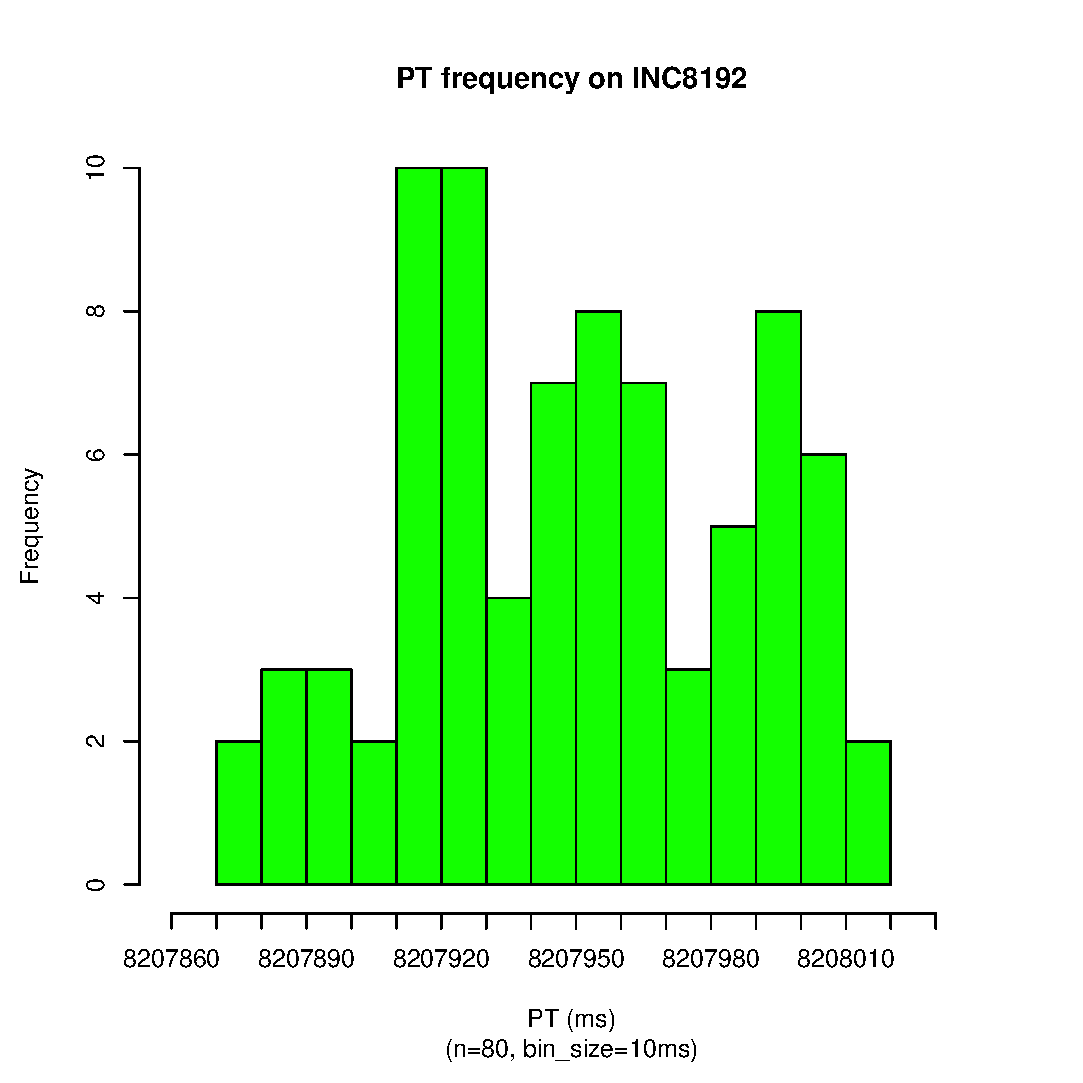
\includegraphics[scale=0.43]{8192_sec_pt_hist.eps}
		\label{fig:put8192_hist1}
	}
	\subfigure[PT frequency on INC16384]{
		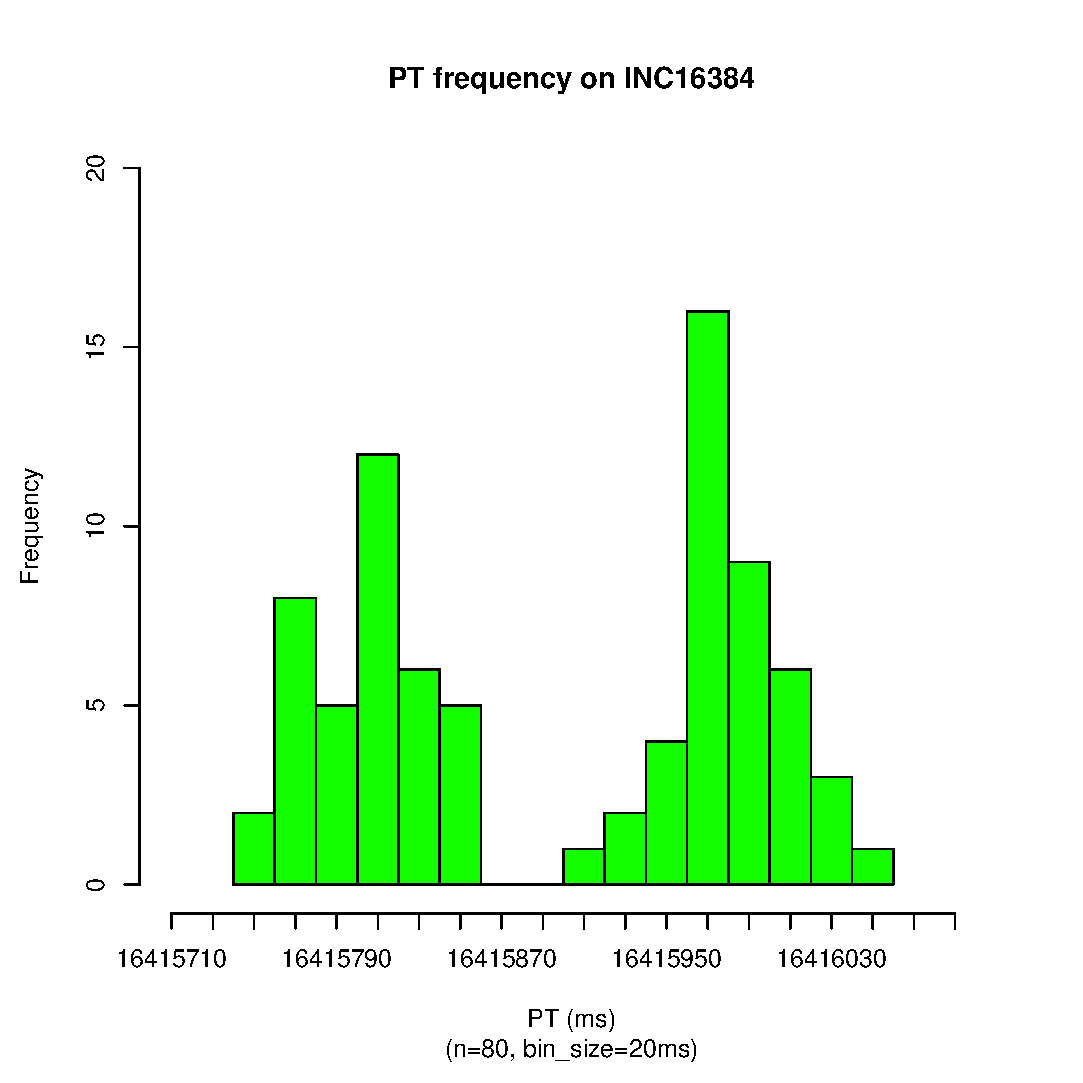
\includegraphics[scale=0.43]{16384_sec_pt_hist.eps}
		\label{fig:put16384_hist1}
	}
	\caption{PT Histograms of INC2048 $...$ INC16384~\label{fig:pt_hist4}}
\end{figure}


\section{Histograms on the EMPv5 Data~\label{sec:empv5_hist}}
The base data of the following histograms are from Table~\ref{tab:exp_notes1}.

\subsection{ET}

\begin{figure}[hp!]
	\centering
	\subfigure[ET frequency on INC1]{
		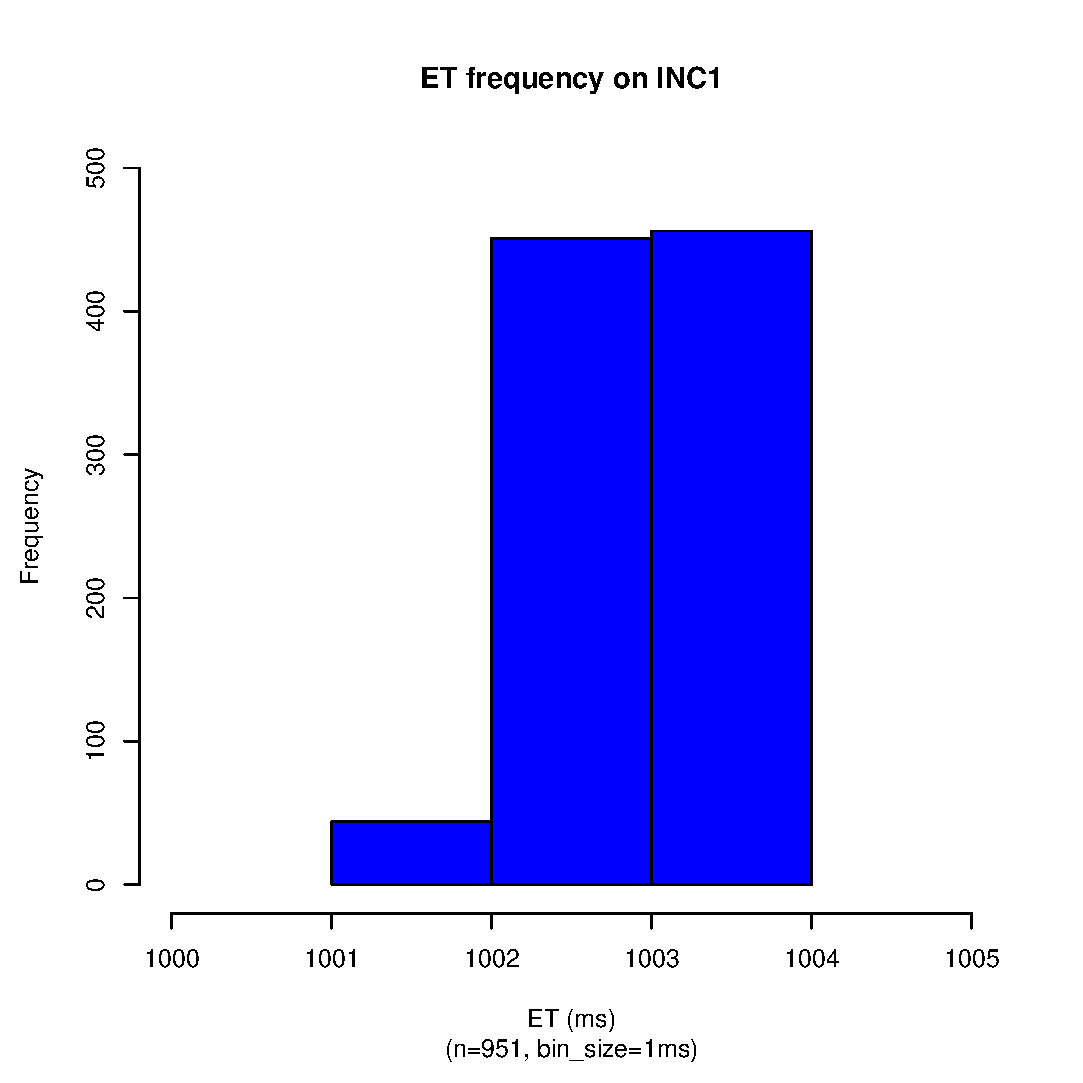
\includegraphics[scale=0.43]{1_sec_et_hist_v5.eps}
		\label{fig:inc1_et_hist_v5}
	}
	\subfigure[ET frequency on INC2]{
		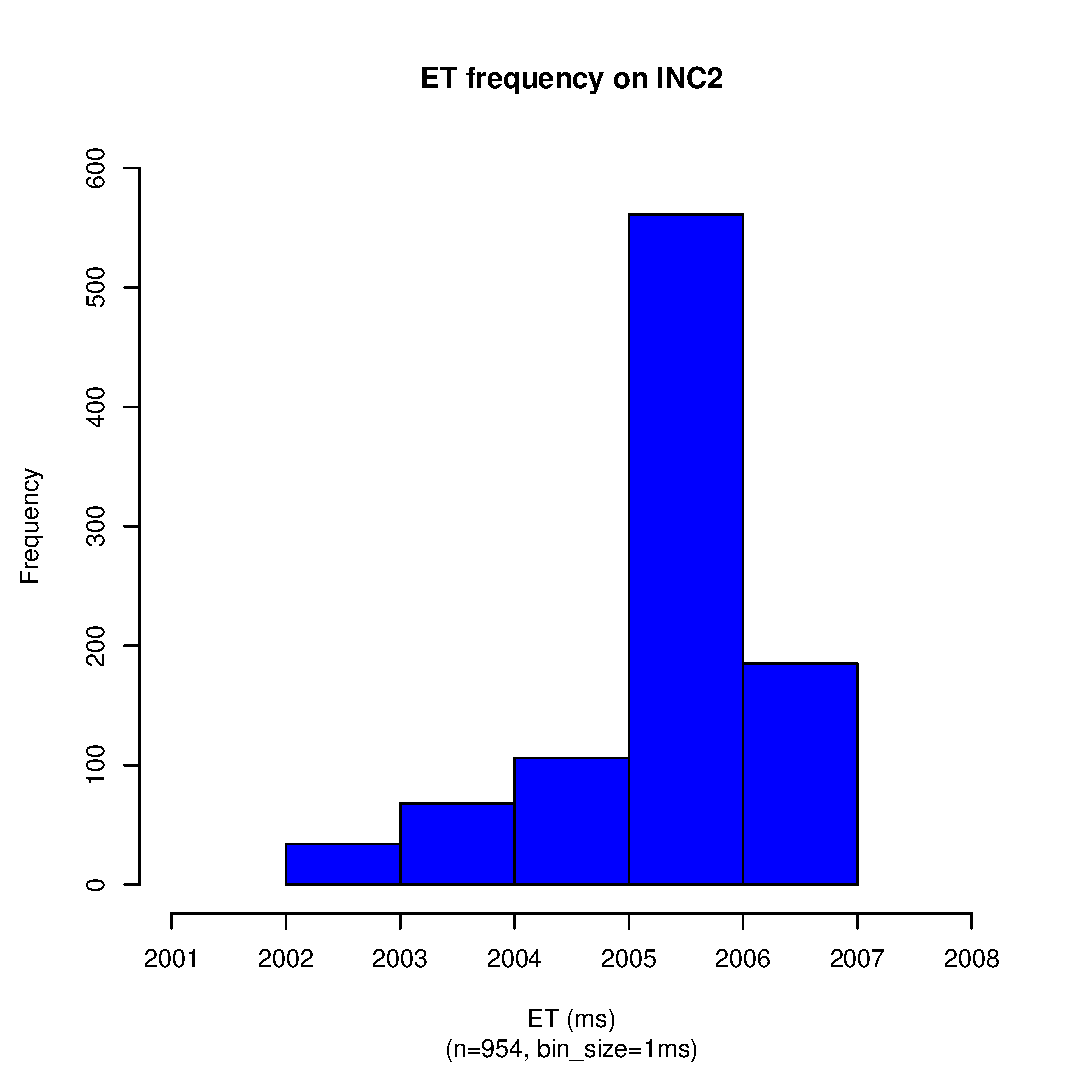
\includegraphics[scale=0.43]{2_sec_et_hist_v5.eps}
		\label{fig:inc2_et_hist_v5}
	}
	\subfigure[ET frequency on INC4]{
		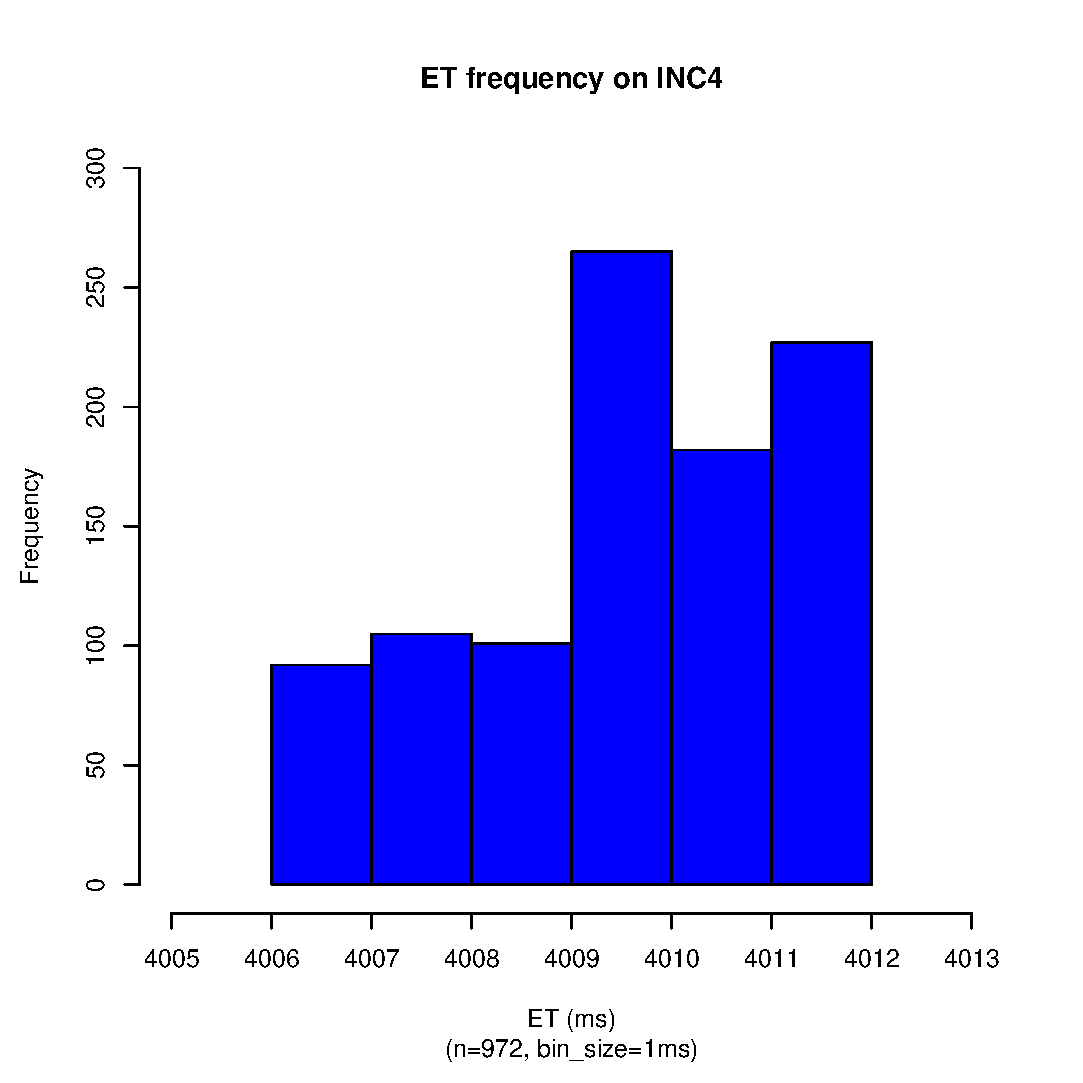
\includegraphics[scale=0.43]{4_sec_et_hist_v5.eps}
		\label{fig:inc4_et_hist_v5}
	}
	\subfigure[ET frequency on INC8]{
		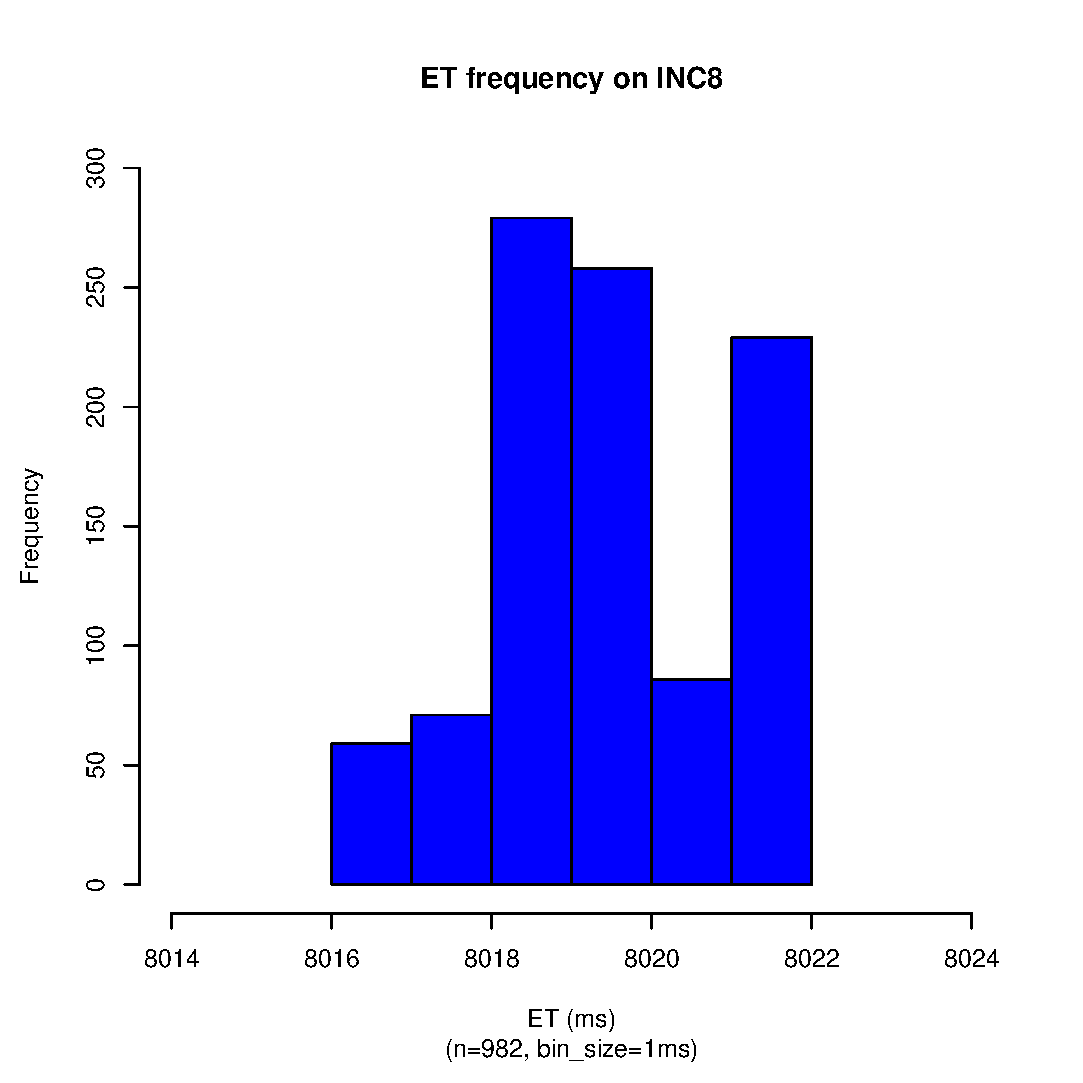
\includegraphics[scale=0.43]{8_sec_et_hist_v5.eps}
		\label{fig:inc8_et_hist_v5}
	}
	\caption{ET Histograms of INC1 ... INC8~\label{fig:et_hist_v51}}
\end{figure}

\begin{figure}[hp!]
	\centering
	\subfigure[ET frequency on INC16]{
		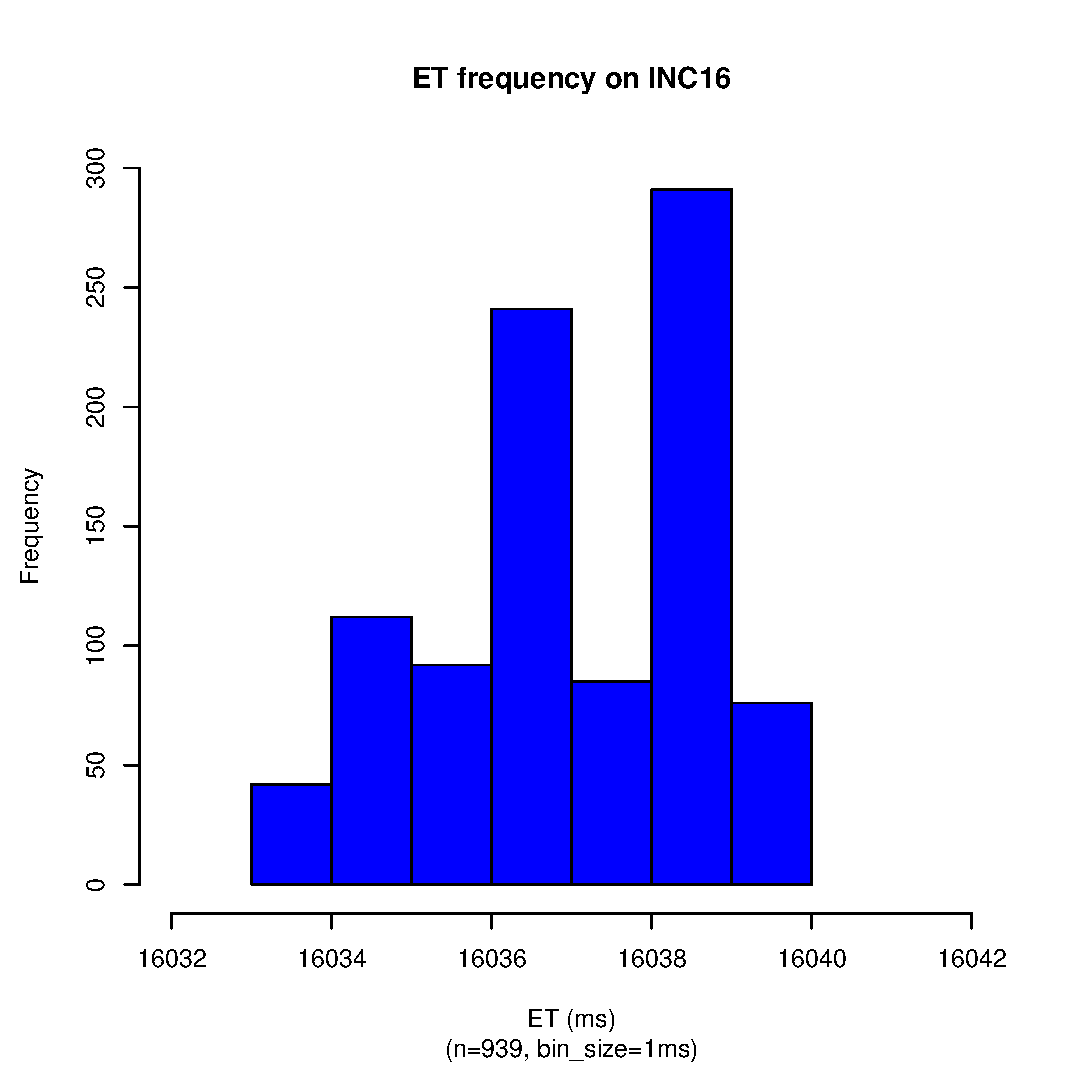
\includegraphics[scale=0.43]{16_sec_et_hist_v5.eps}
		\label{fig:inc16_et_hist_v5}
	}
	\subfigure[ET frequency on INC32]{
		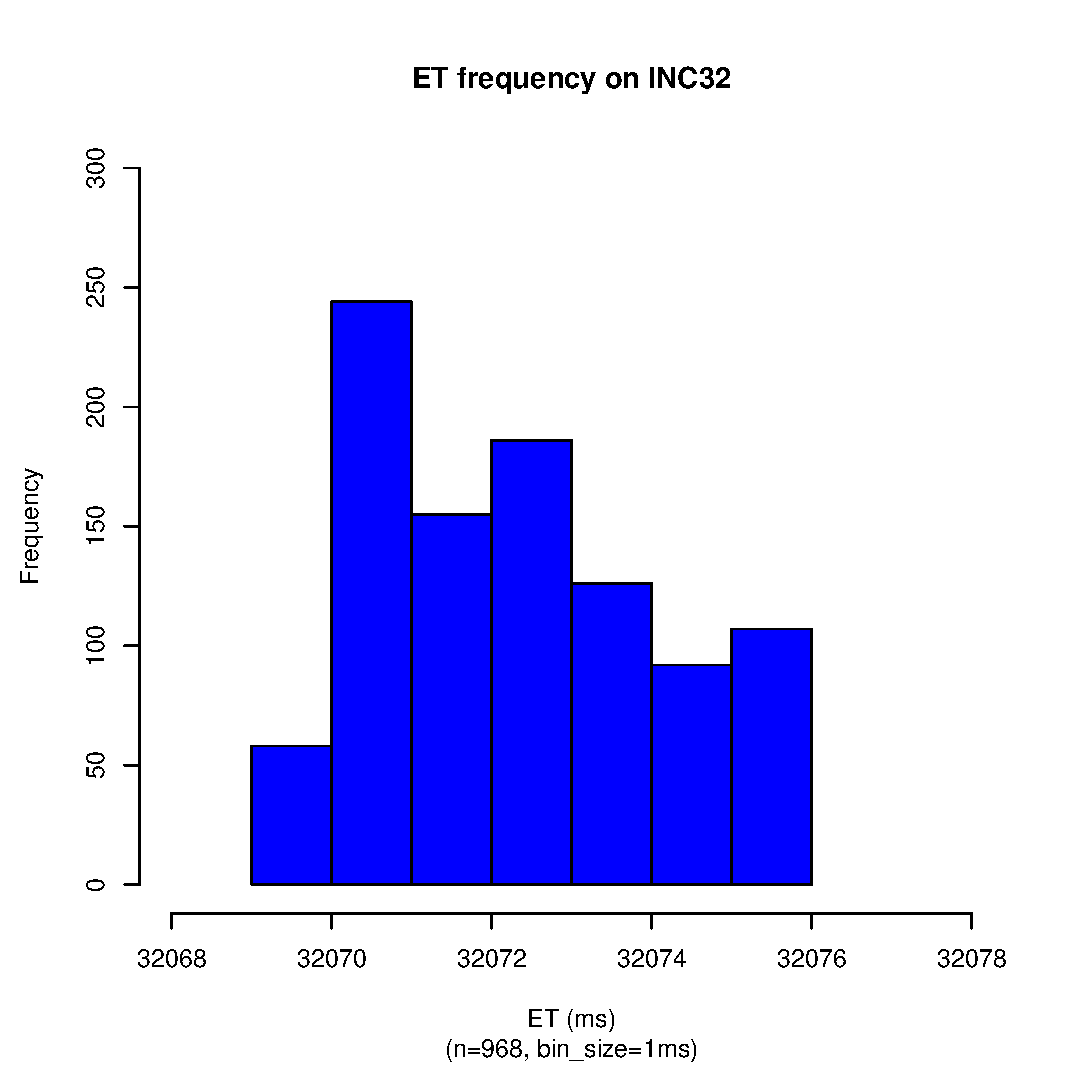
\includegraphics[scale=0.43]{32_sec_et_hist_v5.eps}
		\label{fig:inc32_et_hist_v5}
	}
	\subfigure[ET frequency on INC64]{
		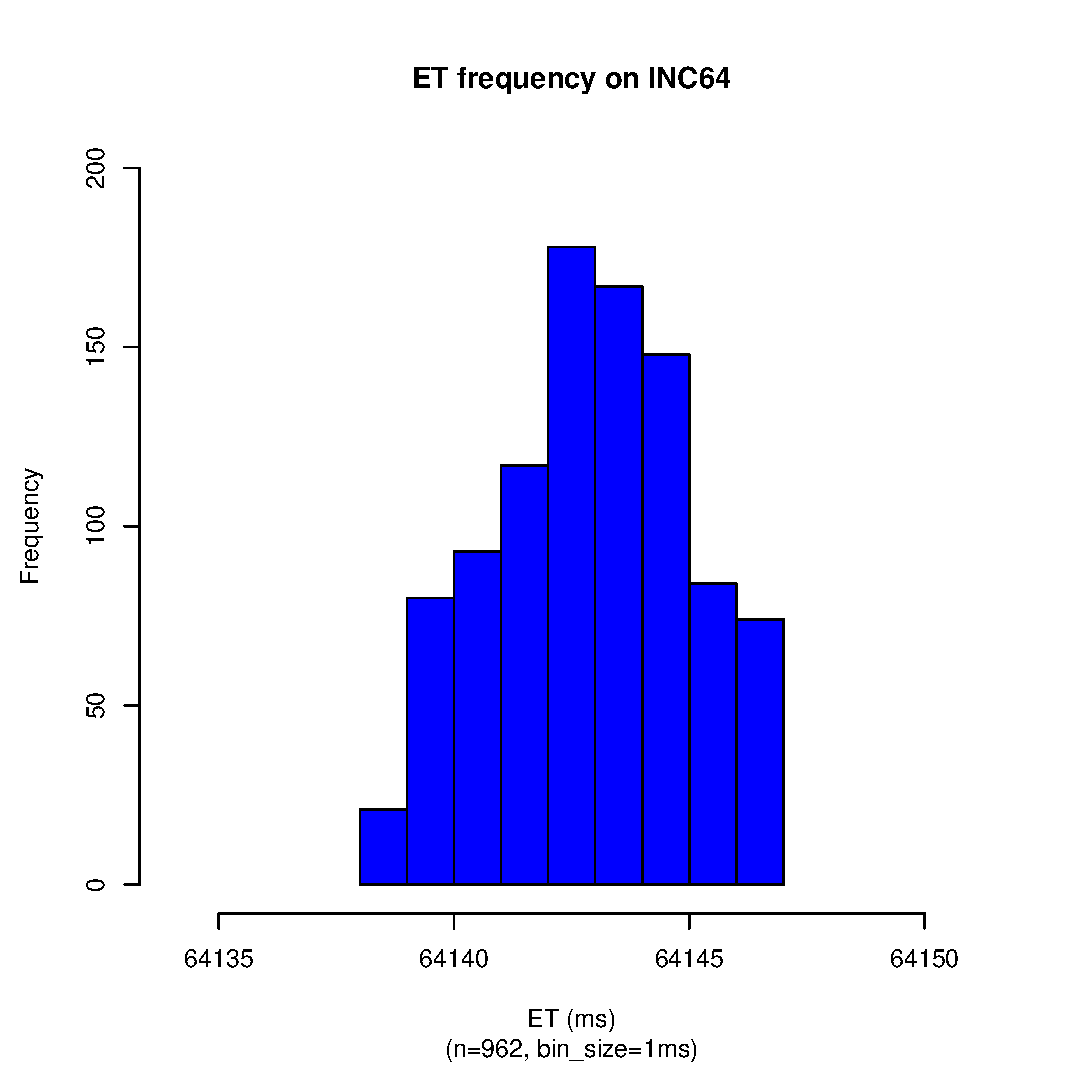
\includegraphics[scale=0.43]{64_sec_et_hist_v5.eps}
		\label{fig:inc64_et_hist_v5}
	}
	\caption{ET Histograms of INC16 ... INC64~\label{fig:et_hist_v52}}
\end{figure}

\newpage

\begin{figure}[hp!]
	\centering
	\subfigure[ET frequency on INC128]{
		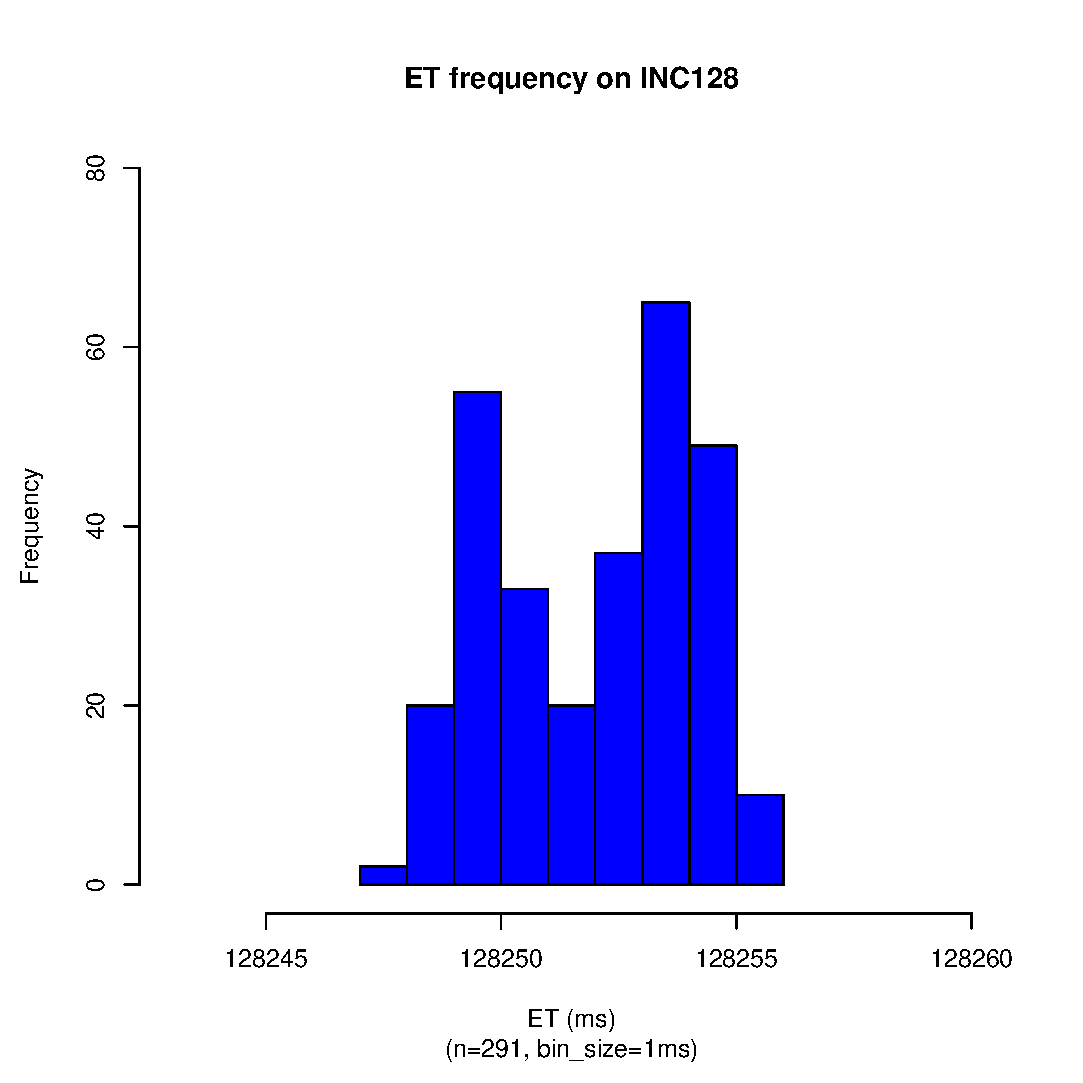
\includegraphics[scale=0.43]{128_sec_et_hist_v5.eps}
		\label{fig:inc128_et_hist_v5}
	}
	\subfigure[ET frequency on INC256]{
		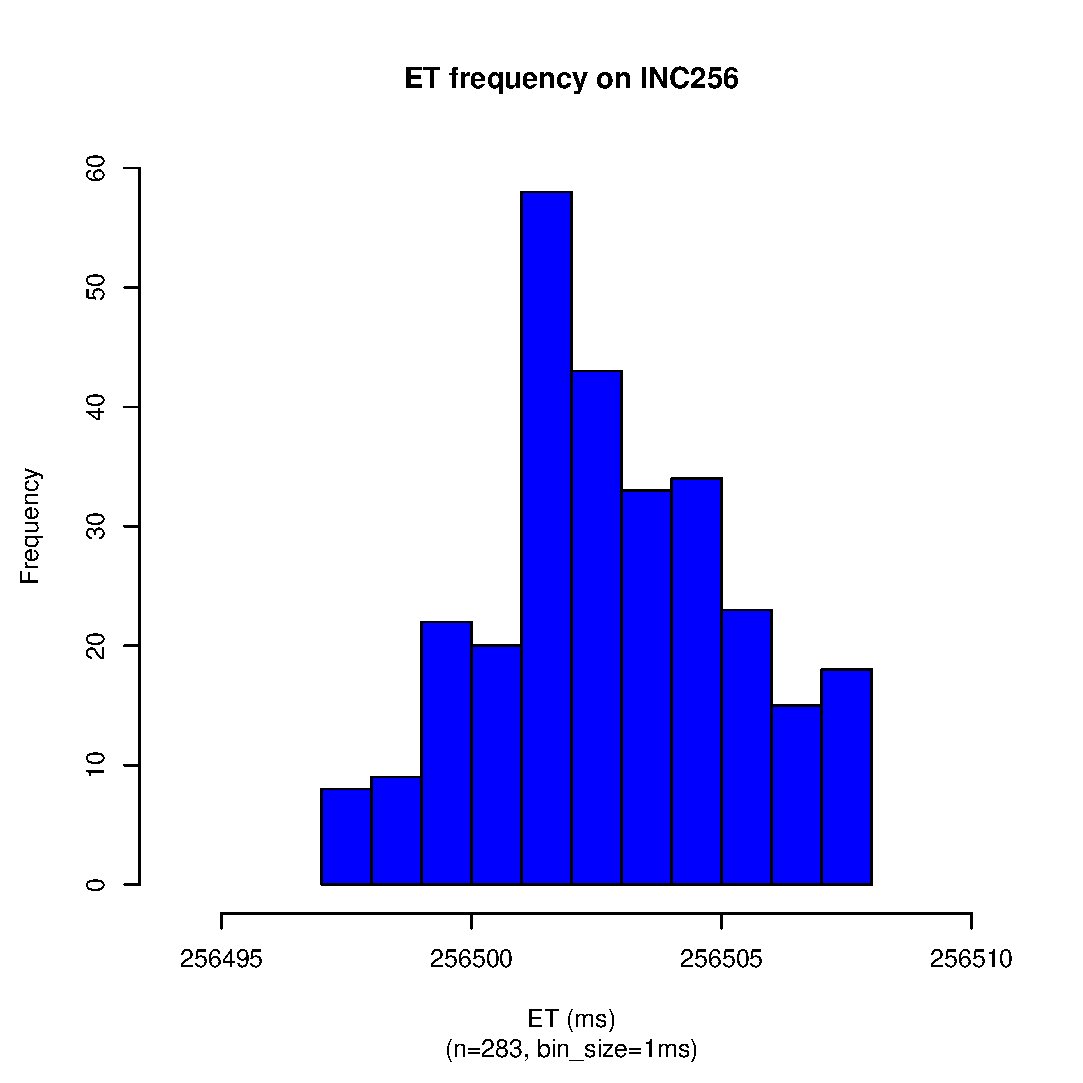
\includegraphics[scale=0.43]{256_sec_et_hist_v5.eps}
		\label{fig:inc256_et_hist_v5}
	}
	\subfigure[ET frequency on INC512]{
		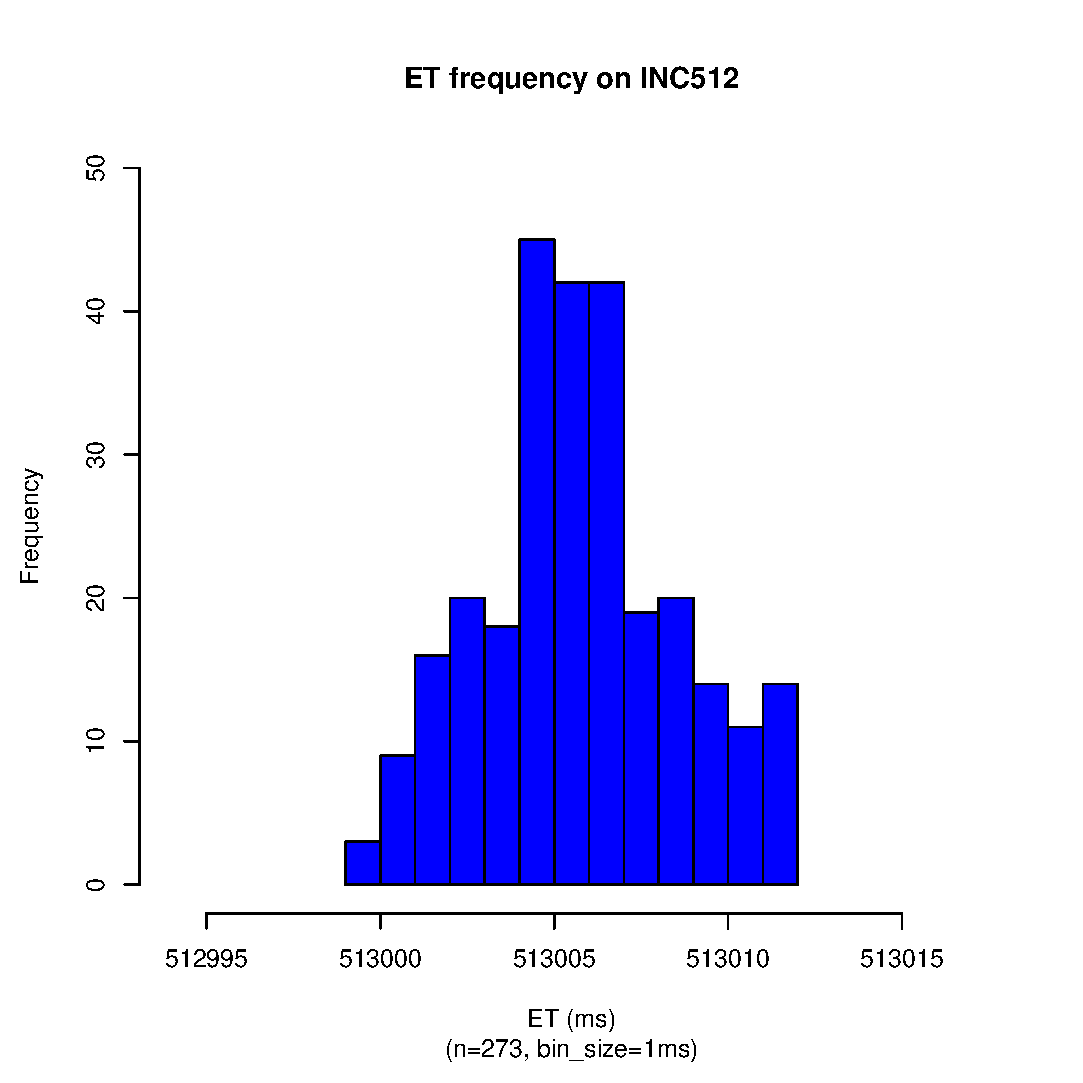
\includegraphics[scale=0.43]{512_sec_et_hist_v5.eps}
		\label{fig:inc512_et_hist_v5}
	}
	\subfigure[ET frequency on INC1024]{
		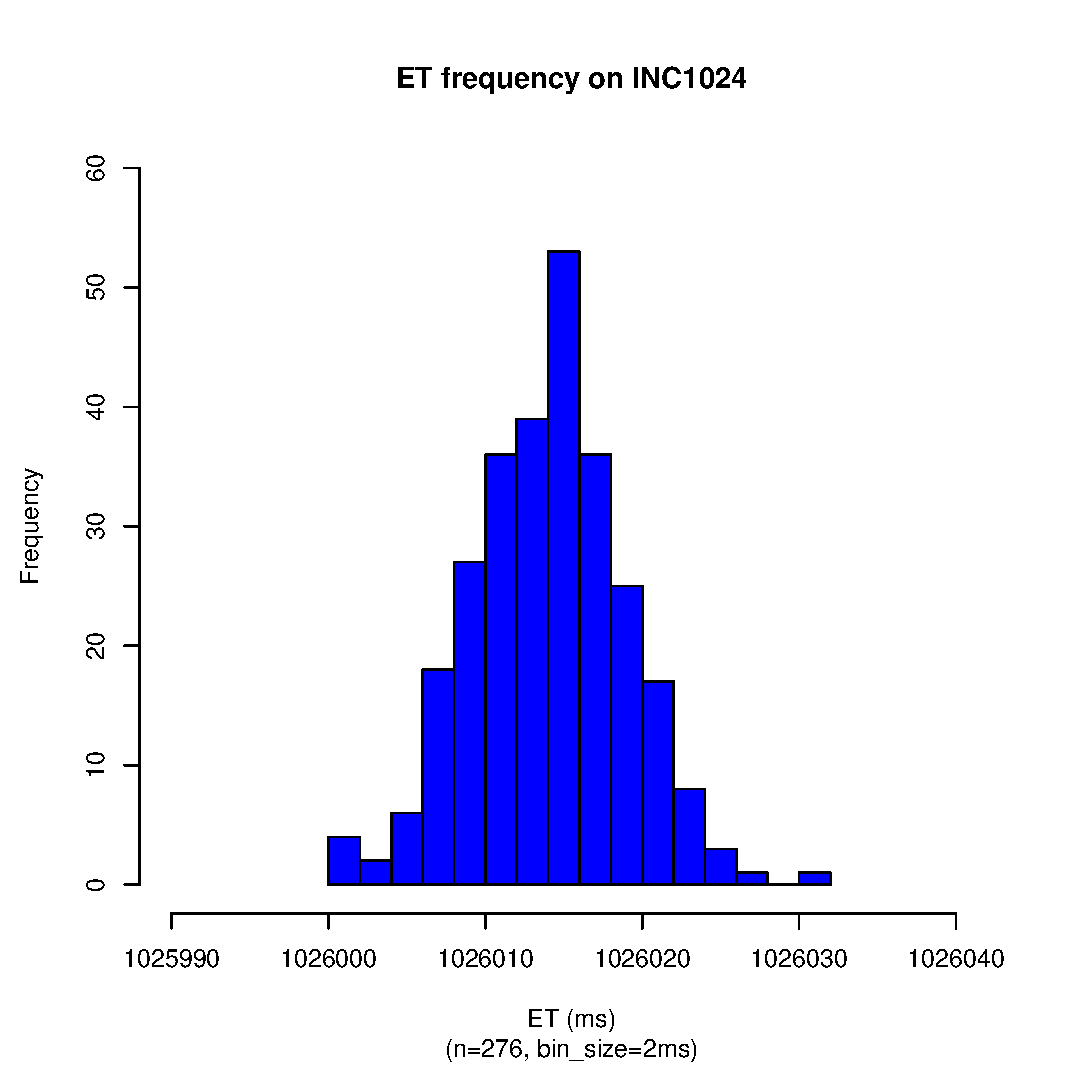
\includegraphics[scale=0.43]{1024_sec_et_hist_v5.eps}
		\label{fig:inc1024_et_hist_v5}
	}
	\caption{ET Histograms of INC128 ... INC1024~\label{fig:et_hist_v53}}
\end{figure}

\newpage

\begin{figure}[hp!]
	\centering
	\subfigure[ET frequency on INC2048]{
		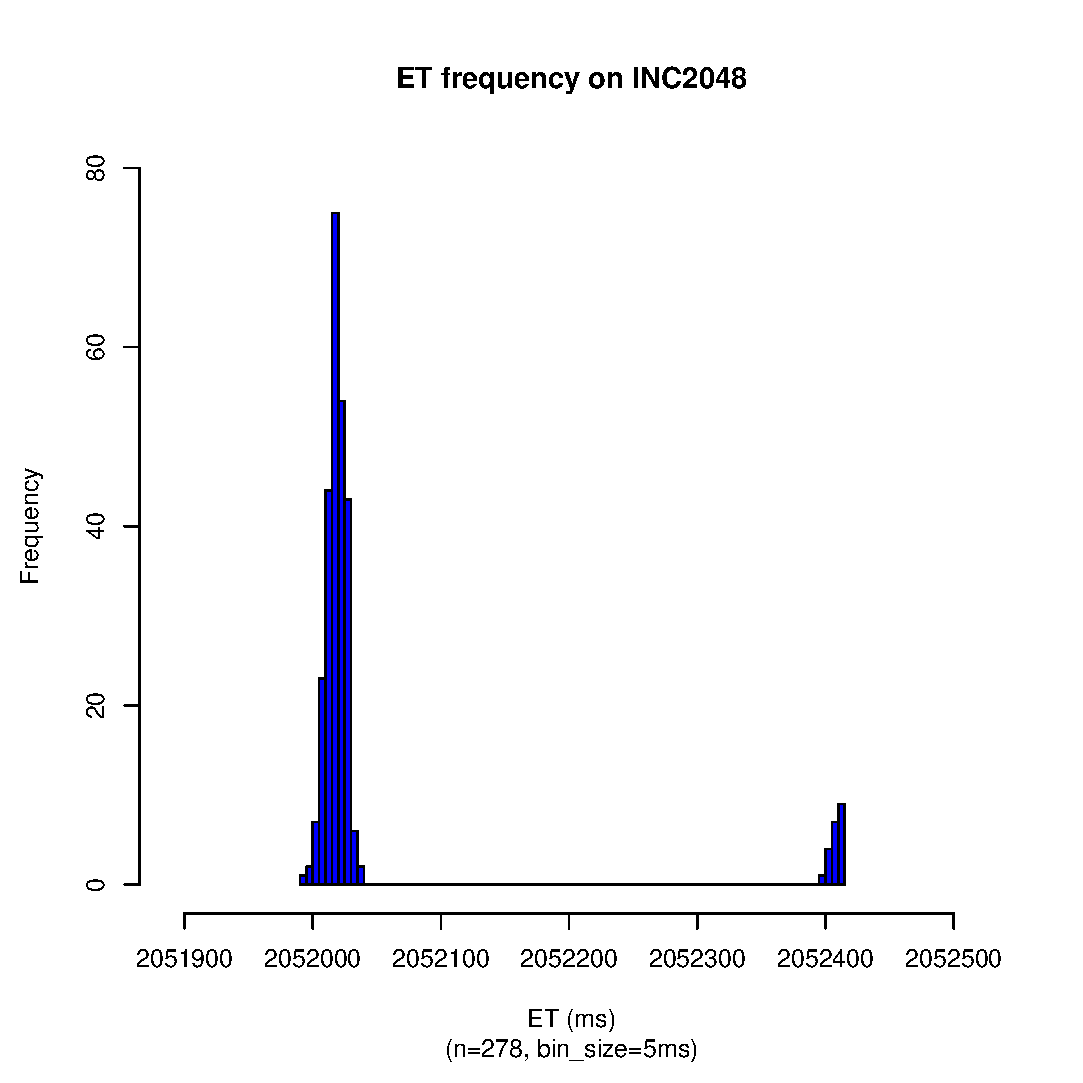
\includegraphics[scale=0.43]{2048_sec_et_hist_v5.eps}
		\label{fig:inc2048_et_hist_v5}
	}
	\subfigure[ET frequency on INC4096]{
		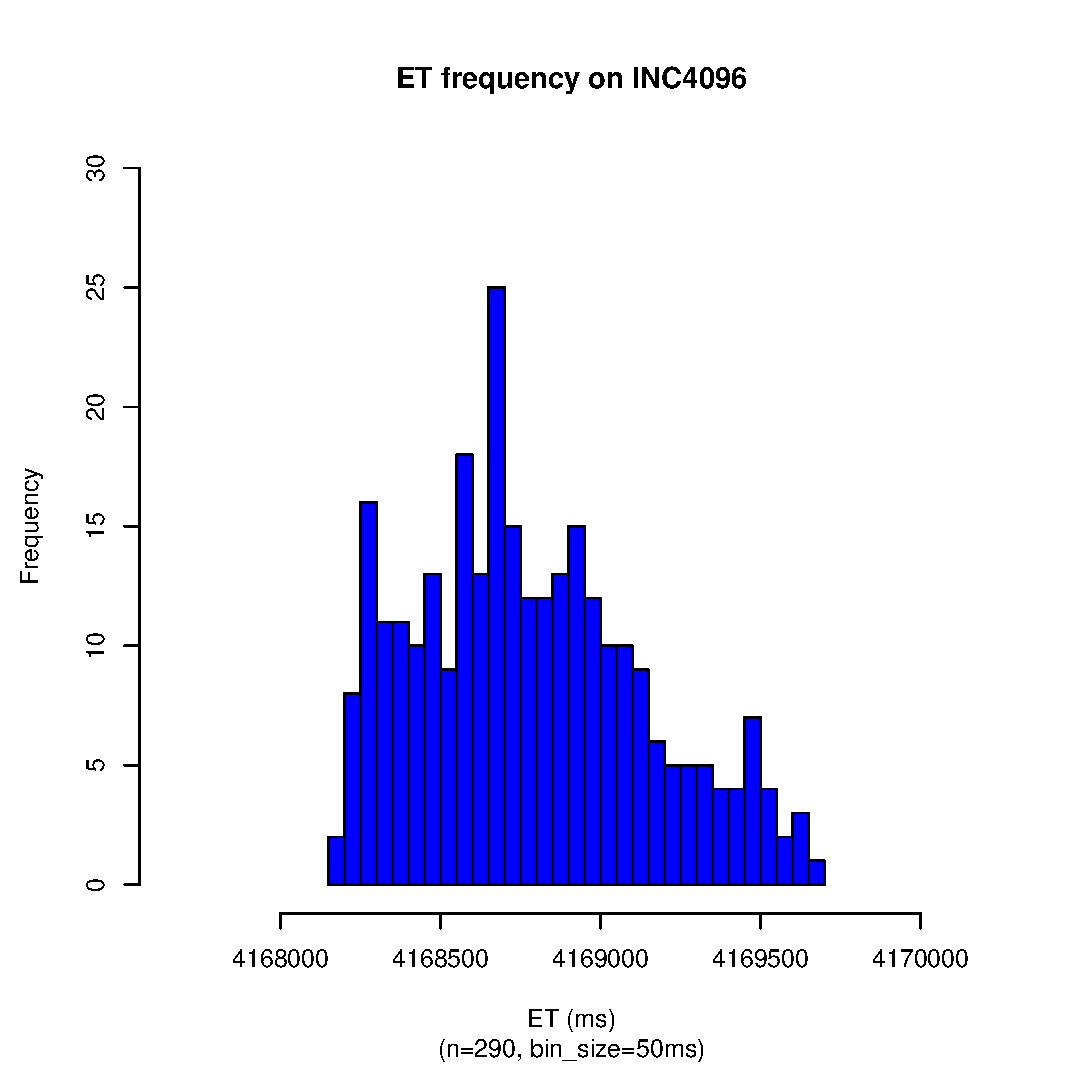
\includegraphics[scale=0.43]{4096_sec_et_hist_v5.eps}
		\label{fig:inc4096_et_hist_v5}
	}
	\subfigure[ET frequency on INC8192]{
		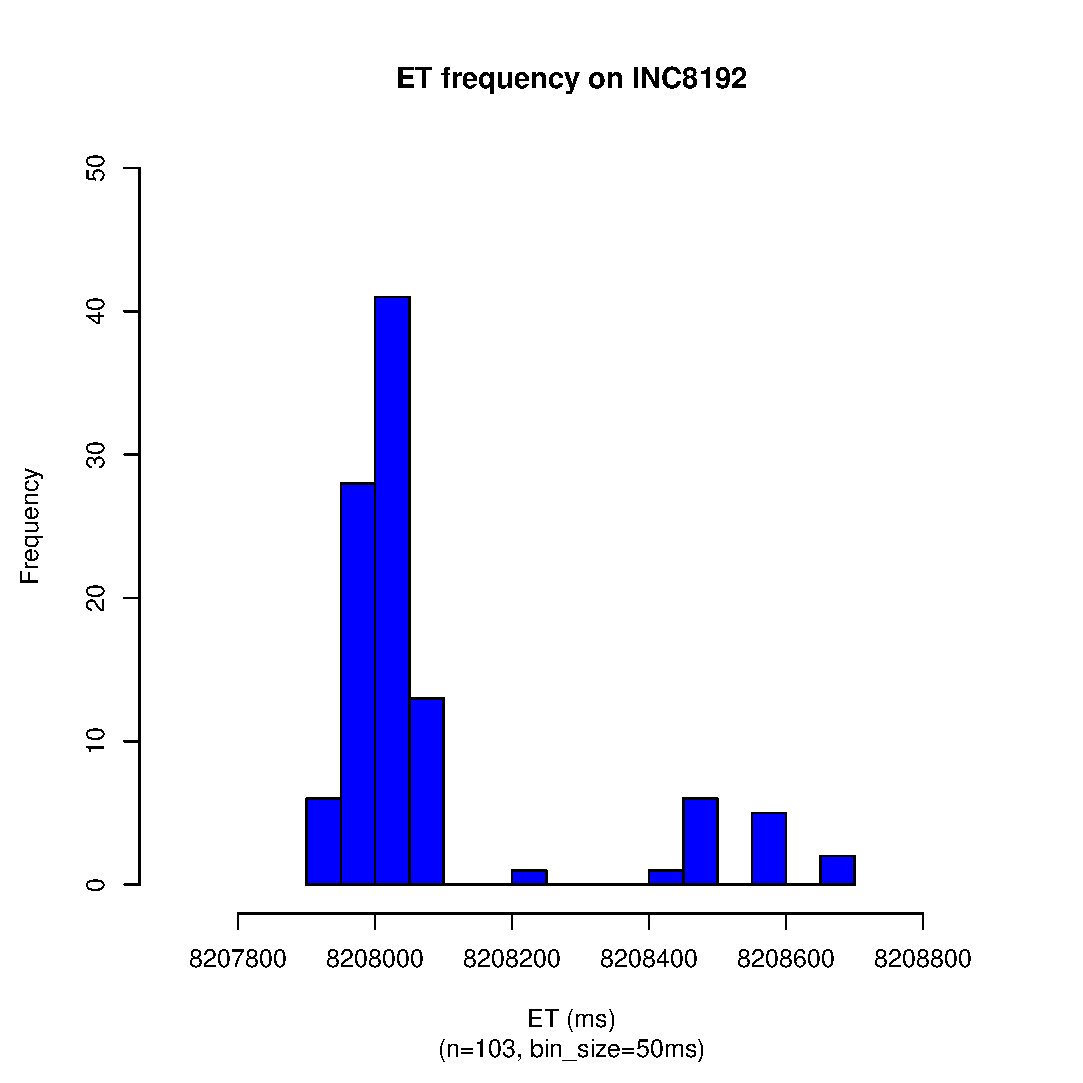
\includegraphics[scale=0.43]{8192_sec_et_hist1_v5.eps}
		\label{fig:inc8192_et_hist_v5}
	}
	\subfigure[ET frequency on INC16384]{
		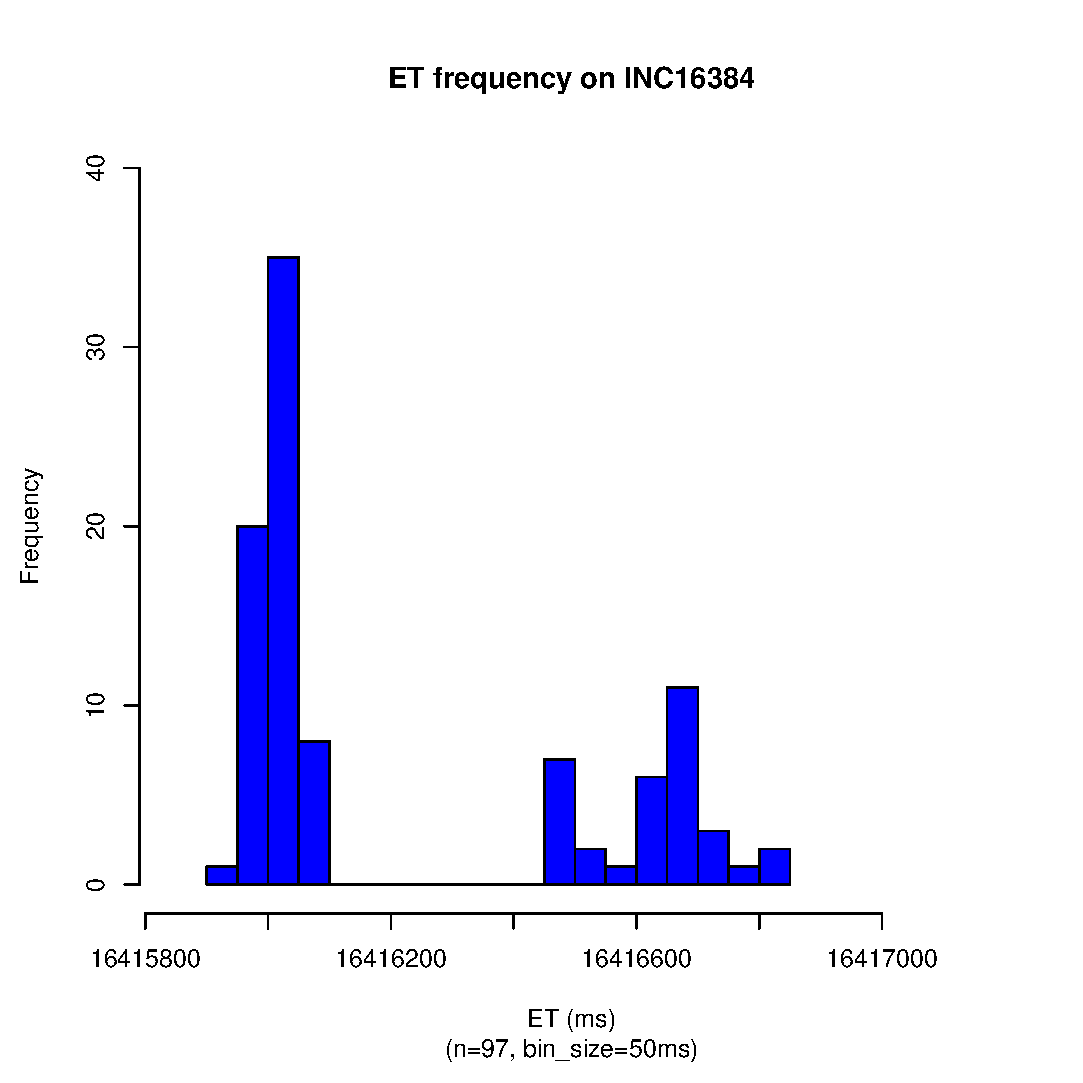
\includegraphics[scale=0.43]{16384_sec_et_hist1_v5.eps}
		\label{fig:inc16384_et_hist_v5}
	}
	\caption{ET Histograms of INC2048 $...$ INC16384~\label{fig:et_hist_v54}}
\end{figure}

\newpage

\subsection{PT}

\begin{figure}[hp!]
	\centering
	\subfigure[PT frequency on INC1]{
		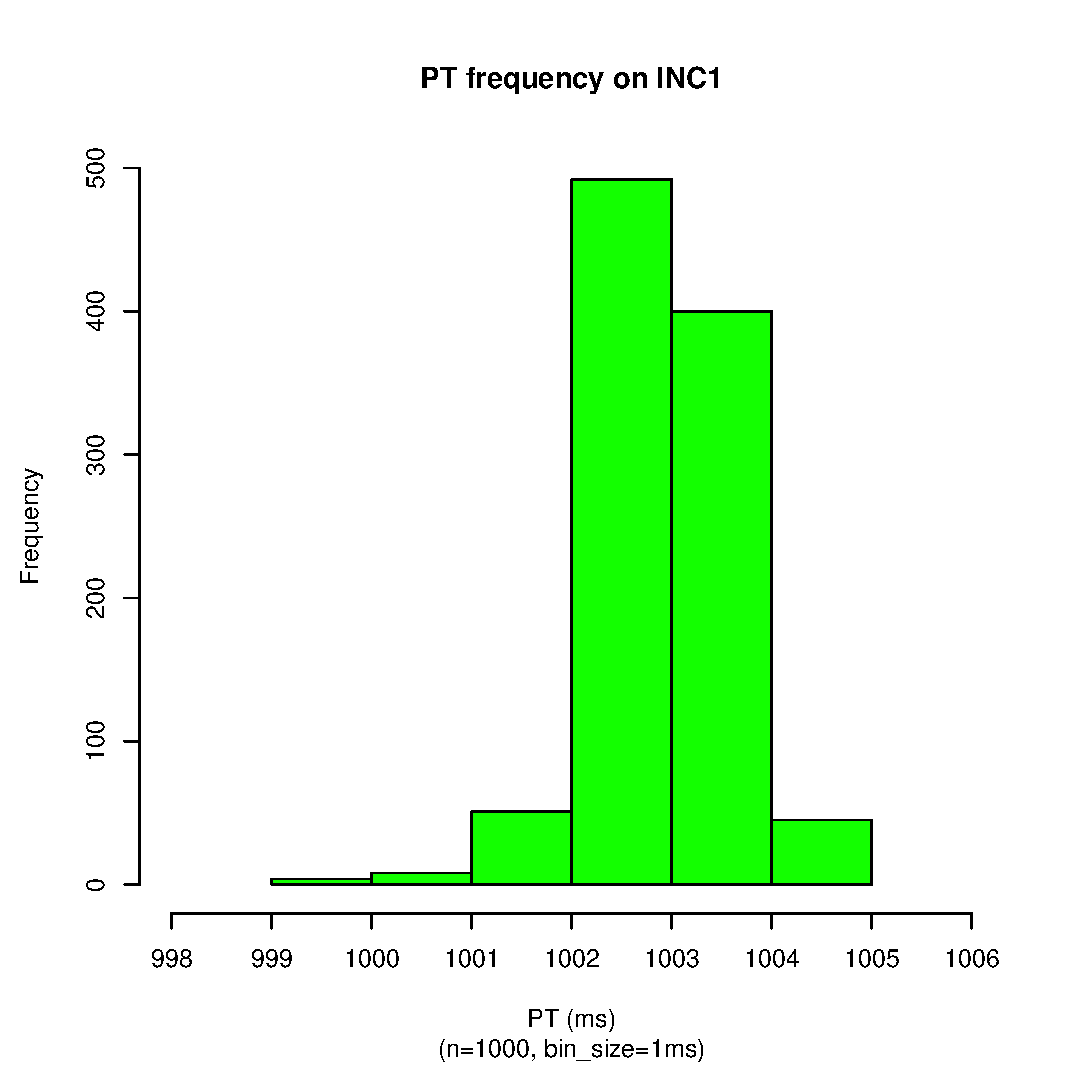
\includegraphics[scale=0.43]{1_sec_pt_hist_v5.eps}
		\label{fig:inc1_hist_v5}
	}
	\subfigure[PT frequency on INC2]{
		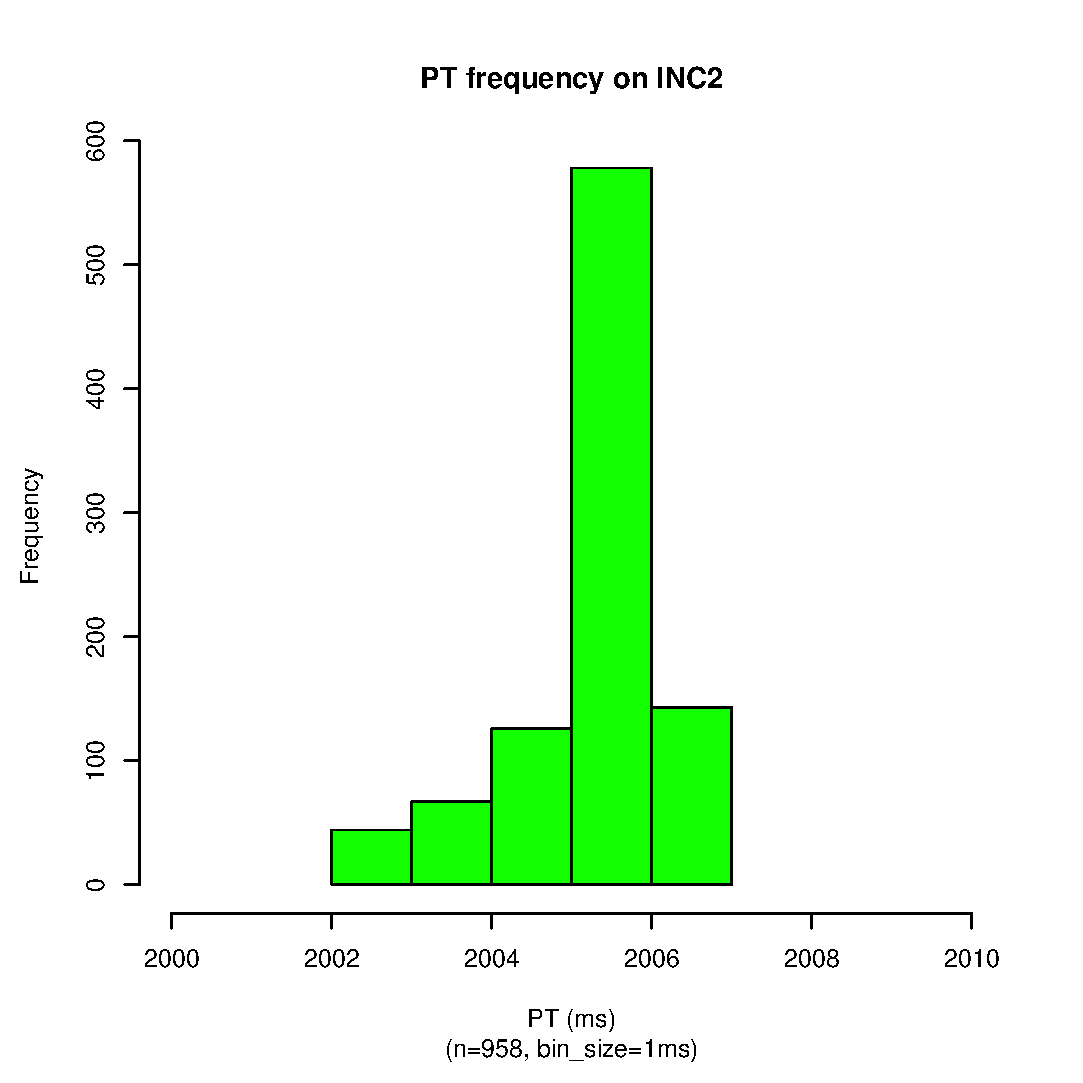
\includegraphics[scale=0.43]{2_sec_pt_hist_v5.eps}
		\label{fig:inc2_hist_v5}
	}
	\subfigure[PT frequency on INC4]{
		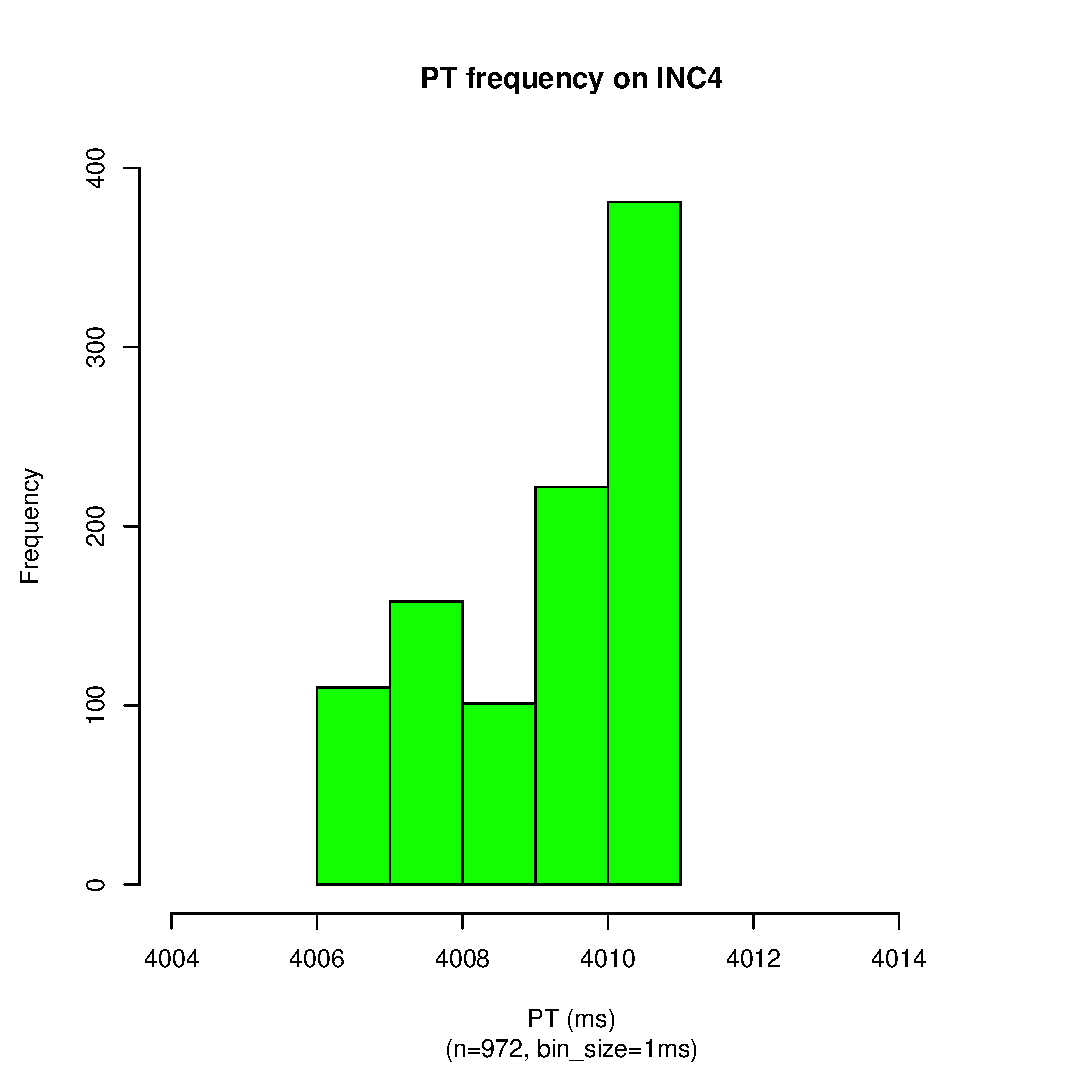
\includegraphics[scale=0.43]{4_sec_pt_hist_v5.eps}
		\label{fig:inc4_hist_v5}
	}
	\subfigure[PT frequency on INC8]{
		\includegraphics[scale=0.43]{8_sec_pt_hist_v5.eps}
		\label{fig:inc8_hist_v5}
	}
	\caption{PT Histograms of INC1 ... INC8~\label{fig:pt_hist_v51}}
\end{figure}

\begin{figure}[hp!]
	\centering
	\subfigure[PT frequency on INC16]{
		\includegraphics[scale=0.43]{16_sec_pt_hist_v5.eps}
		\label{fig:inc16_hist_v5}
	}
	\subfigure[PT frequency on INC32]{
		\includegraphics[scale=0.43]{32_sec_pt_hist_v5.eps}
		\label{fig:inc32_hist_v5}
	}
	\subfigure[PT frequency on INC64]{
		\includegraphics[scale=0.43]{64_sec_pt_hist_v5.eps}
		\label{fig:inc64_hist_v5}
	}
	\caption{PT Histograms of INC16 ... INC64~\label{fig:pt_hist_v52}}
\end{figure}

\newpage

\begin{figure}[hp!]
	\centering
	\subfigure[PT frequency on INC128]{
		\includegraphics[scale=0.43]{128_sec_pt_hist_v5.eps}
		\label{fig:inc128_hist_v5}
	}
	\subfigure[PT frequency on INC256]{
		\includegraphics[scale=0.43]{256_sec_pt_hist_v5.eps}
		\label{fig:inc256_hist_v5}
	}
	\subfigure[PT frequency on INC512]{
		\includegraphics[scale=0.43]{512_sec_pt_hist_v5.eps}
		\label{fig:inc512_hist_v5}
	}
	\subfigure[PT frequency on INC1024]{
		\includegraphics[scale=0.43]{1024_sec_pt_hist_v5.eps}
		\label{fig:inc1024_hist_v5}
	}
	\caption{PT Histograms of INC128 ... INC1024~\label{fig:pt_hist_v53}}
\end{figure}

\newpage

\begin{figure}[hp!]
	\centering
	\subfigure[PT frequency on INC2048]{
		\includegraphics[scale=0.43]{2048_sec_pt_hist_v5.eps}
		\label{fig:inc2048_hist_v5}
	}
	\subfigure[PT frequency on INC4096]{
		\includegraphics[scale=0.43]{4096_sec_pt_hist_v5.eps}
		\label{fig:inc4096_hist_v5}
	}
	\subfigure[PT frequency on INC8192]{
		\includegraphics[scale=0.43]{8192_sec_pt_hist1_v5.eps}
		\label{fig:inc8192_hist_v5}
	}
	\subfigure[PT frequency on INC16384]{
		\includegraphics[scale=0.43]{16384_sec_pt_hist1_v5.eps}
		\label{fig:inc16384_hist_v5}
	}
	\caption{PT Histograms of INC2048 $...$ INC16384~\label{fig:pt_hist_v54}}
\end{figure}


\end{document}